%\documentclass[a4paper,11pt]{memoir} 
\documentclass[oneside, a4paper,11pt]{memoir} 

\usepackage[utf8]{inputenc}
\usepackage[danish]{babel}
\usepackage[T1]{fontenc}
\usepackage[left=4.0cm, right=2.0cm, top=3.0cm, bottom=3.0cm]{geometry} 
\usepackage{amsmath,amssymb}																						

% SIUnitX  http://ctan.org/pkg/siunitx
\usepackage{siunitx,booktabs}		
\sisetup{per=slash}																						
\sisetup{per-mode = reciprocal}
\sisetup{inter-unit-product = \ensuremath{{}\cdot{}}}
\sisetup{output-decimal-marker = {,} }
\DeclareSIUnit{\kroner}{kr.}
\DeclareSIUnit{\LSb}{LSb}
\DeclareSIUnit{\cycles}{cycles}
\DeclareSIUnit{\div}{Div}

\usepackage{graphicx}
\newsubfloat{figure}% Allow subfloats in figure environment
\usepackage{dcolumn,booktabs}
\usepackage{url}
\usepackage{wrapfig}

% Redigere billed-/tabelteksterne.
\usepackage{caption}
\usepackage{subcaption}
\captionsetup{font=small,
labelfont={it,bf},textfont=sf,
format=hang}

% Packages for color handling
\usepackage[usenames,dvipsnames,svgnames,table]{xcolor}

\usepackage{threeparttable}

\usepackage{lscape}

\usepackage{enumitem}

% TODONotes http://ctan.org/pkg/todonotes
\usepackage{todonotes}
\usepackage{placeins}
\usepackage{lastpage}

\usepackage[hidelinks]{hyperref}  
\hypersetup{bookmarks=false}
\hypersetup{pdftitle={Embedded Modul\ae rt Audio Effekt System}} 
\hypersetup{pdfsubject={4. Semester Projekt, F18, Grp. [3]}}
\hypersetup{pdfauthor={J\"{o}rn Jacobi, Emil Schier Christiansen, Henrik Lund Hansen, Jes Rydall Larsen, Sonny Fink, Frederik Halling}}


% For includering af .pdf
\usepackage{pdfpages}

% Bibliografi
\usepackage{babelbib}
\bibliographystyle{abbrv}

% Noget forsideopsætning
\usepackage{soul} % lege lege
\sodef\an{}{0.2em}{.9em plus.6em}{1em plus.1em minus.1em}
\newcommand\stext[1]{\an{\scshape#1}}

% New commands 
\newcommand{\g}{9,82 \si{\meter\per\second\squared}}
\newcommand{\dcite}[1]{\quotedblbase{#1}\textquotedblright}
\newcommand{\husk}[2]{\todo[inline,color=green!40]{#1: #2}}
\newcommand{\jj}[1]{\todo[inline,color=green!40]{JJ: #1}}
\newcommand{\note}[1]{\todo[inline]{#1}}
\DeclareMathOperator{\lapl}{\mathcal{L}}

% Remove paragraph indentation for document
\setlength{\parindent}{0pt}
\newcommand\hcancel[2][black]{\setbox0=\hbox{$#2$}%
	\rlap{\raisebox{.45\ht0}{\textcolor{#1}{\rule{\wd0}{1pt}}}}#2} 

% Listings package
\usepackage{listings}

%Fede overskrifter
\usepackage{kpfonts}
\usepackage{calc}
\setSingleSpace{1.0}
\SingleSpacing
\definecolor{chaptercolor}{gray}{0.8}
% helper macros
%\newcommand\numlifter[1]{\raisebox{-2cm}[0pt][0pt]{\smash{#1}}}
\newcommand\numlifter[1]{\raisebox{-.8cm}[0pt][0pt]{\smash{#1}}}
\newcommand\numindent{\kern37pt}
\newlength\chaptertitleboxheight
\makechapterstyle{hansen}{
  \renewcommand\printchaptername{\raggedleft}
  \renewcommand\printchapternum{%
    \begingroup%
    \leavevmode%
    \chapnumfont%
    \strut%
    \numlifter{\thechapter}%
    \numindent%
\endgroup%
}
  \renewcommand*{\printchapternonum}{%
    \vphantom{\begingroup%
      \leavevmode%
      \chapnumfont%
      \numlifter{\vphantom{9}}%
      \numindent%
      \endgroup}
    \afterchapternum}
  \setlength\midchapskip{0pt}
  \setlength\beforechapskip{0.5\baselineskip}
  \setlength{\afterchapskip}{1\baselineskip}
  \renewcommand\chapnumfont{%
    %\fontsize{3cm}{0cm}%
    \fontsize{2cm}{0cm}
    \bfseries%
    \sffamily%
    \color{chaptercolor}%
  }
  \renewcommand\chaptitlefont{%
    \normalfont%
    %\huge%
    \LARGE%
    \bfseries%
    \raggedleft%
  }%
  \settototalheight\chaptertitleboxheight{%
    \parbox{\textwidth}{\chaptitlefont \strut bg\\bg\strut}}
  \renewcommand\printchaptertitle[1]{%
    \parbox[t][\chaptertitleboxheight][t]{\textwidth}{%
      %\microtypesetup{protrusion=false}% add this if you use microtype
      \chaptitlefont\strut ##1\strut}%
}}
\chapterstyle{hansen}
\aliaspagestyle{chapter}{empty} % just to save some space

%linje afstand
%\DisemulatePackage{setspace}
%\usepackage[nodisplayskipstretch]{setspace}
%\setstretch{0.5}
%\siglespacing
%\onehalfspacing                                       
%\doublespacing

%compile debug, check pdflatex time
\newcommand\showtimer{Timer: \the\numexpr\the\pdfelapsedtime*1000/65536 \relax}
%\pdfresettimer}
%\usepackage{fancyhdr}
%\pagestyle{fancy}
%\fancyfoot[CE,CO]{\showtimer}




\begin{document}
% --------- Frontpage ------------------
\begin{titlingpage}
\thispagestyle{empty}
\centering
{ \setlength{\baselineskip}{24pt}
{\Huge \stext{Embedded Modul\ae rt Audio Effekt System} \par
%\textit{\&}\par
%\stext{Analogier}
}\par
\stext{Indlejrede systemer og signalbehandling - F18}
\vspace*{1cm}



\par

\includegraphics[width=0.5\linewidth]{./billeder/SDU_segl1.png}
\par\vspace*{2\onelineskip}
\stext{4. Semester Projekt}\par

\large\stext{J\"{o}rn Jacobi -- 230674}\par
\large\stext{Emil Schier Christiansen -- ddmmyy}\par
\large\stext{Henrik Lund Hansen -- 270494}\par
\large\stext{Jes Rydall Larsen -- 140893}\par
\large\stext{Sonny Fink -- ddmmyy}\par
\large\stext{Frederik Halling -- ddmmyy}\par

\vfill
\vspace*{2\onelineskip}
\stext{Gruppe 3}\par
\stext{Vejleder: Ib Refer }\par
\stext{1. februar - 25. maj 2018}\hfill
%\stext{24. maj 2013}\hfill
\par\vspace*{2\onelineskip}
\small
\stext{M\ae rsk Mc-Kinney M\o ller Instituttet}\par
\stext{Syddansk Universitet}
\enlargethispage{2\onelineskip}
}
\end{titlingpage}


% --------- Abstract -------------------
\newpage
\thispagestyle{empty}
\renewcommand{\abstractnamefont}{\normalfont\bfseries}
\renewcommand{\abstracttextfont}{\normalfont}
\begin{abstract}
Resumé	
\end{abstract} 

% --------- Thanks ---------------------
%\newpage\thispagestyle{empty}\null\vfill\begin{center}\emph{Thanks note goes here}\end{center}

%---------- Underskrift
%\newpage\thispagestyle{empty}\null
\section*{Underskrifter}
\vspace{3ex} \hfill Underskrevet d. 24/05-2018\\

\newlength{\streg} \setlength{\streg}{0.49\linewidth}
\vspace*{\fill} \rule{\streg}{1pt} \hfill \rule{\streg}{1pt}\\
\begin{minipage}[b]{\streg}
 \centering
 \rule{0pt}{4ex}
 J\"{o}rn Jacobi \\
 {\footnotesize (230674) (jojac11@student.sdu.dk)}
\end{minipage}
\hfill
\begin{minipage}[b]{\streg}
 \centering
 Emil Schier Christiansen \\
 {\footnotesize (ddmmyy) (xxx@student.sdu.dk)}
\end{minipage}

\vspace*{\fill} \rule{\streg}{1pt} \hfill \rule{\streg}{1pt}\\
\begin{minipage}[b]{\streg}
 \centering
 \rule{0pt}{4ex}
 Henrik Lund Hansen \\
 {\footnotesize (ddmmyy) (xxx@student.sdu.dk)}
\end{minipage}
\hfill
\begin{minipage}[b]{\streg}
 \centering
 Jes Rydall Larsen \\
 {\footnotesize (ddmmyy) (xxx@student.sdu.dk)}
\end{minipage}

\vspace*{\fill} \rule{\streg}{1pt} \hfill \rule{\streg}{1pt}\\
\begin{minipage}[b]{\streg}
	\centering
	\rule{0pt}{4ex}
	Sonny Fink \\
	{\footnotesize (ddmmyy) (xxx@student.sdu.dk)}
\end{minipage}
\hfill
\begin{minipage}[b]{\streg}
	\centering
	Frederik Halling  \\
	{\footnotesize (ddmmyy) (xxx@student.sdu.dk)}
\end{minipage}\newpage\thispagestyle{empty}\null\vfill

%---------- Forord
\newpage
\thispagestyle{empty}
\chapter*{Forord}\label{chap:forord}
\addcontentsline{toc}{chapter}{Forord}
Dette projekt er udarbejdet af seks ingeniør-studerende på 4. semester for Elektronik og Datateknik på Syddansk Universitet. 
Projektet er udført i perioden d. 1. februar til d. 25. maj 2018. 
Projektet er udført under vejledning af Ib Refer. Gruppen takker for støtten gennem forløbet. 

\husk{NOTE}{I nogle rapporter ønsker forfatterne at indsætte et forord. Dette kan være i form af en tak til
	samarbejdspartnere, en dedikation af projektet til bestemte personer, eller fordi de ønsker at
	redegøre for ændrede forhold i forbindelse med rapporten.
	Et forord er ikke en obligatorisk del af et projekt. Det er som navnet siger ”før ordet”, dvs. før selve
	rapporten og kan ofte udelades.}

\subsection{Læsevejledning}
Rapporten bør læses fra start til slut som et samlet og sammenhængende værk. 
Som udgangspunkt antages det, at læseren har et fagligt kompetenceniveau som en studerende på 4. semester med linjefag indenfor elektronik og datateknik.

\subsection{Typografiske konventioner}
Her er en kort oversigt over de typografiske konventioner der anvendes i denne rapport.

\bigskip

\begin{tabular}{l p{0.6\linewidth}}
	\textit{Kursiv tekst}			& Angiver filnavne i den tilhørende kodebase samt fremhævelse af ord eller fagudtryk. \\
	\textbf{Fed tekst}				& Bruges til a fremhæve produkt eller system specifikke betegnelser.\\
	\texttt{Konstant brede tekst}	& Anvendes til kildekode eksempler. Ligeledes anvendes afgrænsende områder.\\
	\emph{Fremhævet tekst}		    & Bliver brugt når der gives en kort introduktion til hvert kapitel.\\
\end{tabular}

\subsection{Typografi}
Rapporten er fremstillet i \LaTeX - Memoir, sat i 11 pt. Computer Modern.\\
Antal sider : \pageref{LastPage}

% Removed for single page
%\newpage\thispagestyle{empty}\null\vfill

%---------- Indholdsfortegnelse  ---
\newpage
\tableofcontents*		

% Removed for single page										
%\newpage

%\DoubleSpacing	
%---------- Kalibrerings side --------
%\input{config/kalib}
%\newpage

%---------- Indledning -------------
\chapter{Indledning}
\vspace*{0.5 cm}
\emph{Kapitel intro}

\section{Formål}
\begin{itemize}
	\item Et projekt er semester krav som man går til eksamen.
	\item Hvor faglighederne indgår.
\end{itemize}

Formålet med projektet er at undersøge hvordan lyd kan behandles og manipuleres ved at bruge digital signalbehandling i et embedded miljø.
Hvordan samples signaler korrekt.
Løsningen skal opbygges som en modulær løsning, således at nye "lydmoduler" kan efter udvikles.
Styringen af modulerne skal kunne forgå igennem EMP boardet - her tænkes det at kunne anvende HID styringen dette board stiller til rådighed og som sammen LCDen skal udgøre en platform til UI'en. 


\section{Problemformulering}


\begin{itemize}
	\item Realtids lydbehandling 
	\item Digital filter design
	\item Analog filter design
	\item OS krav / design
	\item Test krav og eftervisning af forventede
\end{itemize}

\section{Projektafgrænsning}
\begin{itemize}
	\item Produktet er ikke udviklet som et slutprodukt.
\end{itemize}

\section{Kravspecifikation} 
\begin{itemize}
	\item Der skal anvendes vores ARM Cortex-M4 TI launchpad 
	\item Sampling Fs = 44,1 kHz Stereo (CD standard)
	\item FreeRTOS anvendes som OS	 
\end{itemize}

\section{Løsningsmodel}

\section{Proces- og arbejdsmetode}
							

\listoftodos
%\input{config/howto} 

%---------- Chapter ----------------
\chapter{Analoge filtre}\label{kap:filtre}
\vspace*{0.5 cm}
\emph{I dette kapitel vil valg, design og dimensioneringen af løsningens anti-aliasning og rekonstruktions filter blive gennemgået}


%---------- Parts ----------------
%	\item Begrundelse baseret på antal op-amp / orden (6/8)
%	\item Kort teoretisk gennemgang af den valgte topologi
%	\item Beregninger og dimensionering af 6. ordens chebycheb filtre
%	\item Implementeringsvalg og design af hardware/schematics
%\end{itemize}


\section{Analoge filtres rolle ved digital signalbehandling}\label{sec:filter_intro}
\begin{wrapfigure}[30]{r}{3.5cm}
	\vspace{-.5cm}
	\centering
	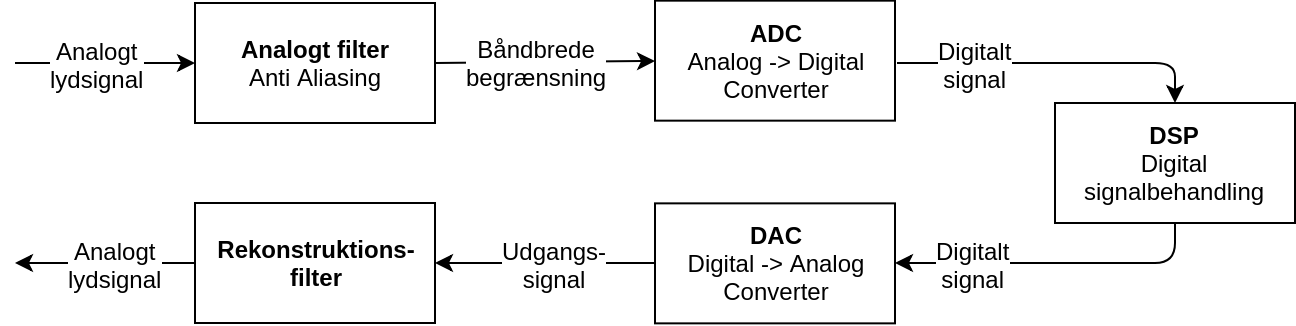
\includegraphics[width=2.5cm]{billeder/dsp_model.png}
	\caption{DSP model.}
	\label{fig:dsp_model}
\end{wrapfigure}

For at kunne udfører digital signalbehandling af et analogt signal, bliver man nød til at overfører signalet fra den analoge verden til den digitale og tilbage igen - dette sker ved sampling og rekonstruktion.
Denne signalbehandling følger nogle faste deltrin, som kan ses i et generelt signal-blok diagram i figur \ref{fig:dsp_model}.
I dette kapitel vil fokus ligge på de analoge signaler og filtre, således vil vigtigheden de analoge filtre blive kortlagt og den efterfølgende analyse og dimensionering  \\

Når et 
\jj{hvad var jeg ved at skrive her ???}

Som udgangspunkt blev opløsningen af den Analog-Digital Converter (ADC) til at vurdere hvor meget dæmpning er analogt filter skulle have for at kunne sikre en komplet og tabsfri gengivelse af signalet.

Ud fra de fremsatte krav til projektet, benyttes der en   microcontroller fra Texas Instruments \cite{spmu296} der er udstyret med en 12bit ADC på de analoge indgange.
For at bestemme opløsning på ADC'en, kan den unipolære\footnote{Unipolær kvanteficering skyldes ADC'ens spændingsområde på $0 \longmapsto \num{3.3}\si{\volt}$.} kvanteficering $\Delta_{ADC}$ bestemmes samt Signal to Noise Ratio $SNR_Q$.
   
\begin{align}
	\Delta_{ADC} &= \frac{V_{max}}{2^N} = \frac{\num{3.3}\si{\volt}}{2^{12}} \approx \num{80.6}\si{\milli\volt}\\
	SNR_Q &= 6,02 N + 2 [\si{\decibel}] = 6,02\cdot 12+2 = 74,24 \si{\decibel} 
\end{align}
 


\note{Kort teoretisk intro til hvorfor filtre skal anvendes til sampling}
\note{Båndbrede begrænsning}
\note{Shannons sampling theorem}
\note{Generel intro til audio signaler}
\note{begrundelse for orden af filter i intro}

\section{Analyse af filter typer}\label{sec:filter_analyse}
%\note{Gennem gang af de filter topologier der har været i betragtning som en mulig løsning.}
For at kunne finde frem til et passende lavpasfilter som antialiasing filter, bliver 4 tilter typer sammenlignet - Butterworth, Chebyshev type I og II samt Bessel (Thomson).
Hver af disse filtre har en tilhørende amplitudekarakteristik der beskrives med følgende overføringsfunktion\cite{anfilter}.

\begin{align} 
H_{butterworth}(j\omega_n) &= \frac{1}{\sqrt{1 + \omega_n^{2n}}} \label{eq:H_butt} \\
H_{bessel} (j\omega_n) &= \frac{H}{a_0 + \omega^2 + ja_1\omega_n} \label{eq:H_bes}\\
H_{chebychevI}(j\omega_n) &= \frac{1}{\sqrt{1 + \epsilon^2 C_n^2(\omega_n)}} \label{eq:H_cheb1} \\
H_{chebychevII}(j\omega_n) &= \frac{1}{\sqrt{1 + \frac{1}{\epsilon^2 C_n^2(\omega_n)}}} \label{eq:H_cheb2} \\
C_n(\omega_n) &=  
\begin{matrix}
	\cos(n\arccos(\omega_n)) & 0 \le \omega_n \le 1 \\  \cosh(n \arccosh(\omega_n)) & 1 \le \omega_n 
\end{matrix} \label{eq:chev_cn_funk}
\end{align}

I ligning (\ref{eq:chev_cn_funk}) fremgår den indre funktion $C_n(\omega_n)$ som bruges i Chebychev I og II i ligening (\ref{eq:H_cheb1}) og (\ref{eq:H_cheb2}).

Figur \ref{fig:filter_typer} viser en samlet fremstilling af amplitude karakteristikken $H(j\omega_n)$ og gruppeløbstiden $D(\omega_n)$ for de fire filtertyper.

\begin{figure}[h!]
	\centering
	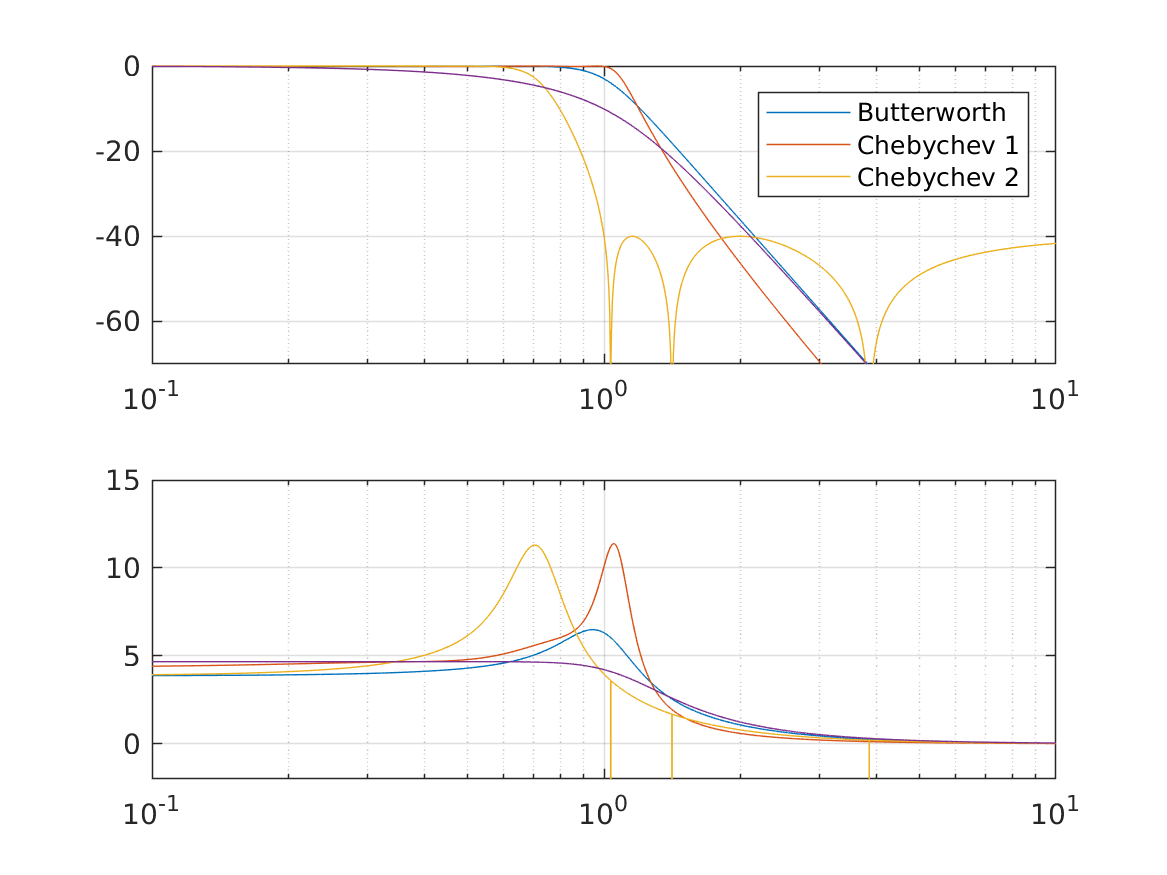
\includegraphics[width=1\textwidth]{matlab/filter_compare.png}
	\caption{Normeret 6.ordens filter karakteristik (øverst) og guppeløbstid (nederst) for filtertyperne Butterworth, Chebychev Type I ($0,1 \si{\decibel}$ rippel) \& Type II ($-40 \si{\decibel}$ stopbånds rippel) og Bessel.}
	\label{fig:filter_typer}
\end{figure}

Det ønskede filter skal have en rimelig flad karakteristisk i pasbåndet og en stejl overgang til stopbåndet.
Således kan lydsignalets amplitude holdes konstant i hele det ønskede frekvensområde da uønsket dæmpning/forstærkning af lydsignalet kan medfører hørbare ændringer af lydbilledet, på samme måde som en equalizer påvirker et lydsignal. 

Ligeledes ønskes en rimelig konstant gruppeløbetid. 
Gruppeløbetiden, der er defineret i ligning (\ref{eq:groupdelay_def})\cite{anfilter}, er et udtryk for hvor stor tidsforsinkelsen på signal som funktion af frekvensen er.

\begin{align}
	D(\omega) \stackrel{def}{=} - \dfrac{d(arg(N(\omega)))}{d\omega}\label{eq:groupdelay_def}
\end{align}

Hvis signal forsinkelsen bliver for stor i et givet frekvensområde, vil der fremstå en hørbar ændring af lydbilledet.
Dette fenomen er dog ret subjektivt og der findes mange meninger om hvilke tærskelværdier der kan accepteres.
Ud fra en lettere gennemgang inden for området, er antages en acceptabel relativ tidsforsinkelse på $D_{rel}(\omega) < -10 \si{\milli\second}$ til projektet.   

\subsection{Valg af filter topologi}
Hvis man som udgangspunkt kun fokusere på filtrenes gruppeløbstid, ville man skulle vælge et Bessel filter.
Bessel filteret, det er designet som et filter med maksimal fald fase, har dog langt fra den ønskede dæmpning i overgangsbåndet.
Det vælges at anvende et Chebychev type I filter, der viser sig at have den bedste dæmpning i overgangsbåndet.
Det høje udsving på gruppeløbetiden for denne filtertype, som det fremgår nederst i figur \ref{fig:filter_typer}, vil på det denomaliserede filter ligger indenfor, de i projektet, acceptable værdier. 
\\
I figur \ref{fig:filter_cheb1_denorm} ses den denormaliserede filterkarakteristik for det valgte filter med en pasbåndsrippel på $0,1 \si{\decibel}$ og en knækfrekvens på $f_c = 18 \si{\kilo\hertz}$. 

\begin{figure}[h!]
	\centering
	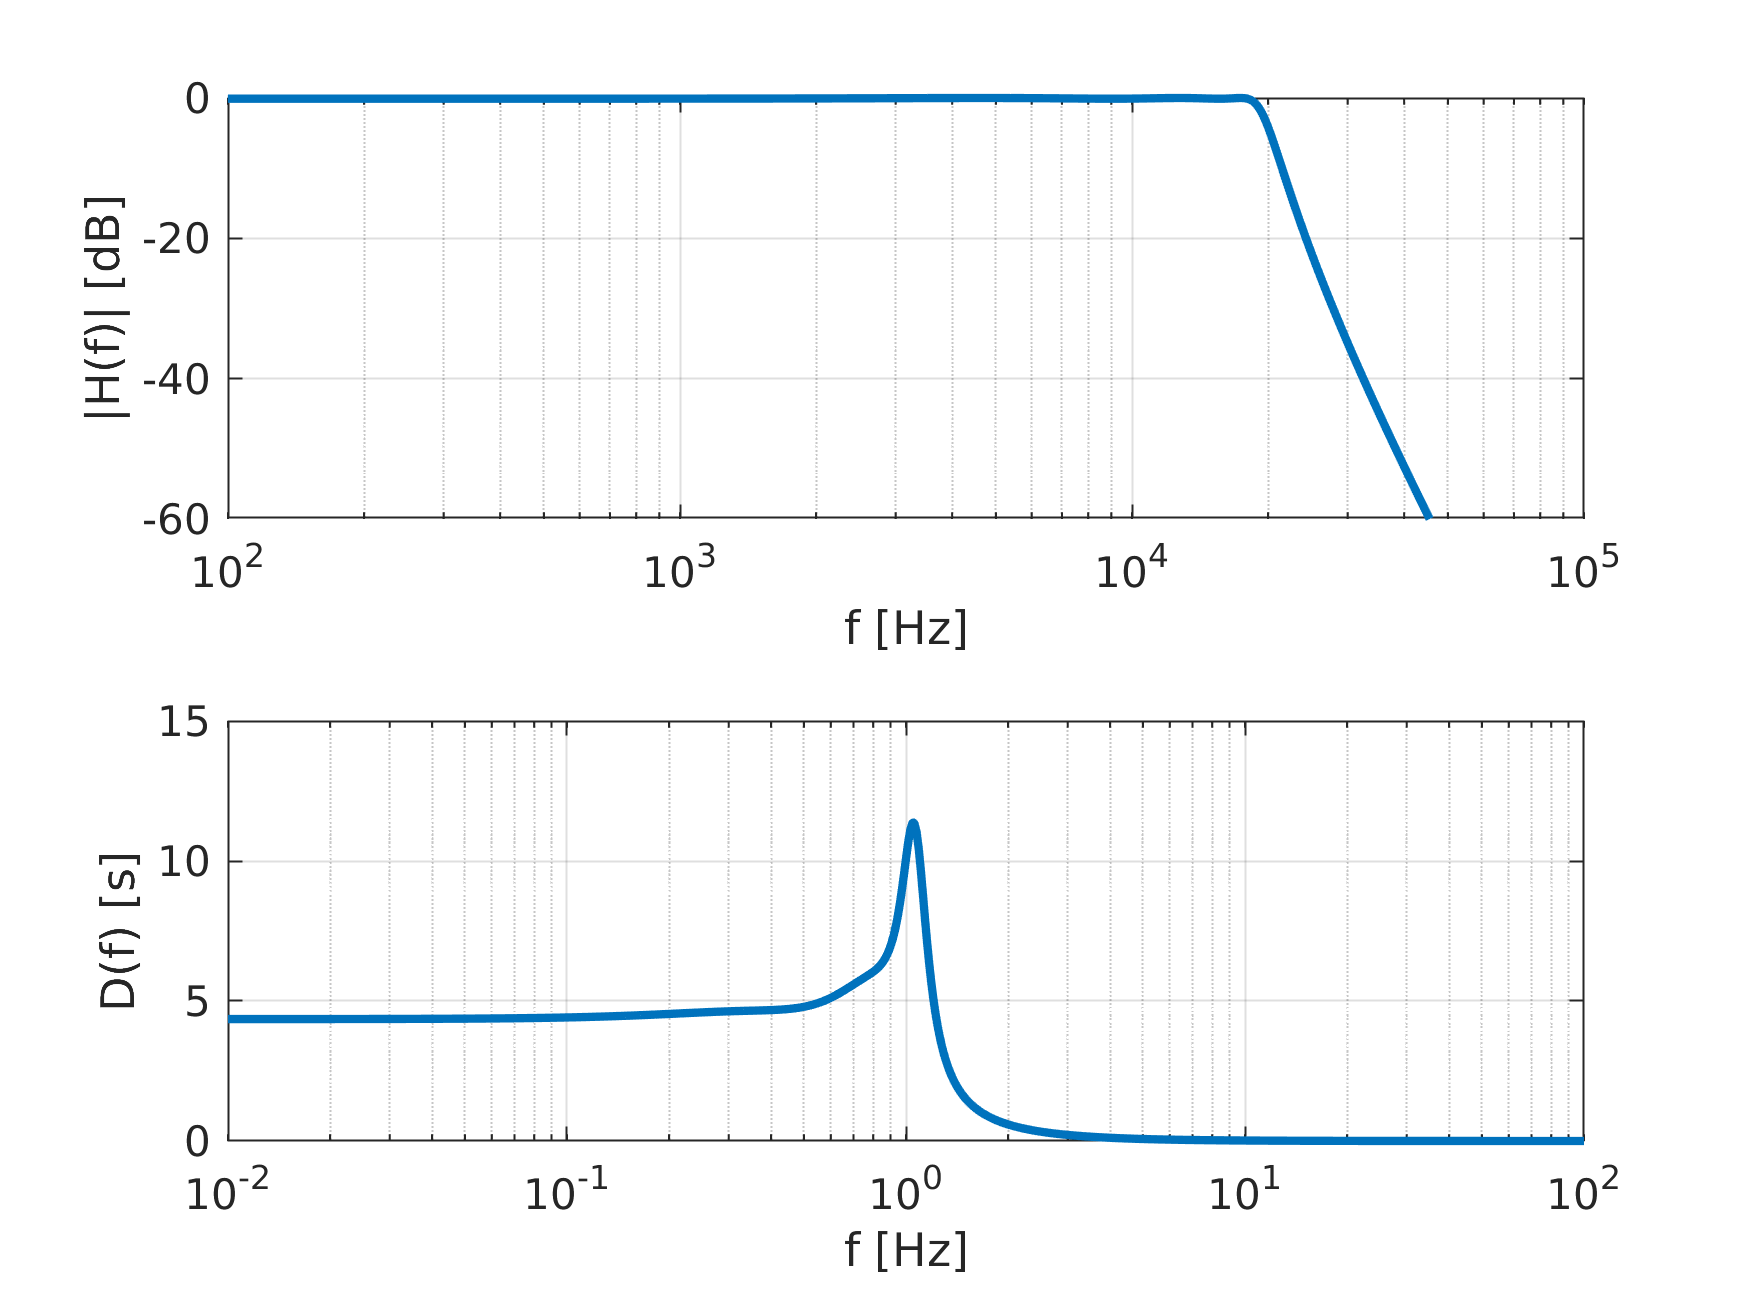
\includegraphics[width=1\textwidth]{matlab/filter_cheb1_denorm.png}
	\caption{Denormeret 6.ordens filter karakteristik og guppeløbstid af Chebyshev Type I ($0,1 \si{\decibel}$}
	\label{fig:filter_cheb1_denorm}
\end{figure}
\jj{ret matlab fil med denormineret grpdelay}

For at kunne bestemme dæmpningen af de demormaliserede filter, findes udtrykket for $|H(f)|$.
Med udgangspunkt i ligning \ref{eq:H_cheb1}, bestemmes $\epsilon$, som er bestemt ved ud fra rippelfaktoren i et Chebyshev filter\footnote{Figur 1.11.1 og ligning 1.11.3 i kilde \cite{anfilter}}
\begin{align}
	K_p = 20 \log \frac{1}{\sqrt{1+\epsilon^2}} \Leftrightarrow \epsilon = \sqrt{10^{K_p/10}-1}
\end{align}
Med en maksimal rippel på $K_p = 0,1 \si{\decibel}$ fås en $\epsilon$ på 
\begin{align}
	\epsilon = \sqrt{10^{0,1/10}-1} = \num{0.1526}
\end{align}

Da det ønskes at beregne $|H(f)|$ i området $f > f_c$ anvendes $C_n$ fra ligning \ref{eq:chev_cn_funk} hvor $w_n > 1$
Dæmpningen ved nyquistfrekvensen på $f_s/2 = \num{22.05}\si{\kilo\hertz}$ kan nu bestemmes som

\begin{align}
|H(f)|_{\si{\decibel}} &= 20 \log \frac{1}{\sqrt{1+ \epsilon^2  \left[\cosh(n \arccosh k )\right]^2 }} \quad, \quad k = \frac{f}{f_c} \\
|H(22,05\si{\kilo\hertz})|_{\si{\decibel}} &= 20 \log \frac{1}{\sqrt{1+ 0,1526^2  \left[\cosh(n \arccosh \frac{22,05\si{\kilo\hertz}}{18\si{\kilo\hertz}} )\right]^2 }} = \num{-12.2568} \si{\decibel}
\end{align}

\subsection{Forventet aliasing ved valgte filter type}
\jj{lidt mere intro til aliasing}
I figur \ref{fig:filter_f_fs} ses amplitude karakteristikken $|H(f)|$ af det valgte filter med blåt og den første periodiske gentagelse af frekvens spektrum $|H(f-f_s)|$ med rødt.
\begin{figure}[h!]
	\centering
	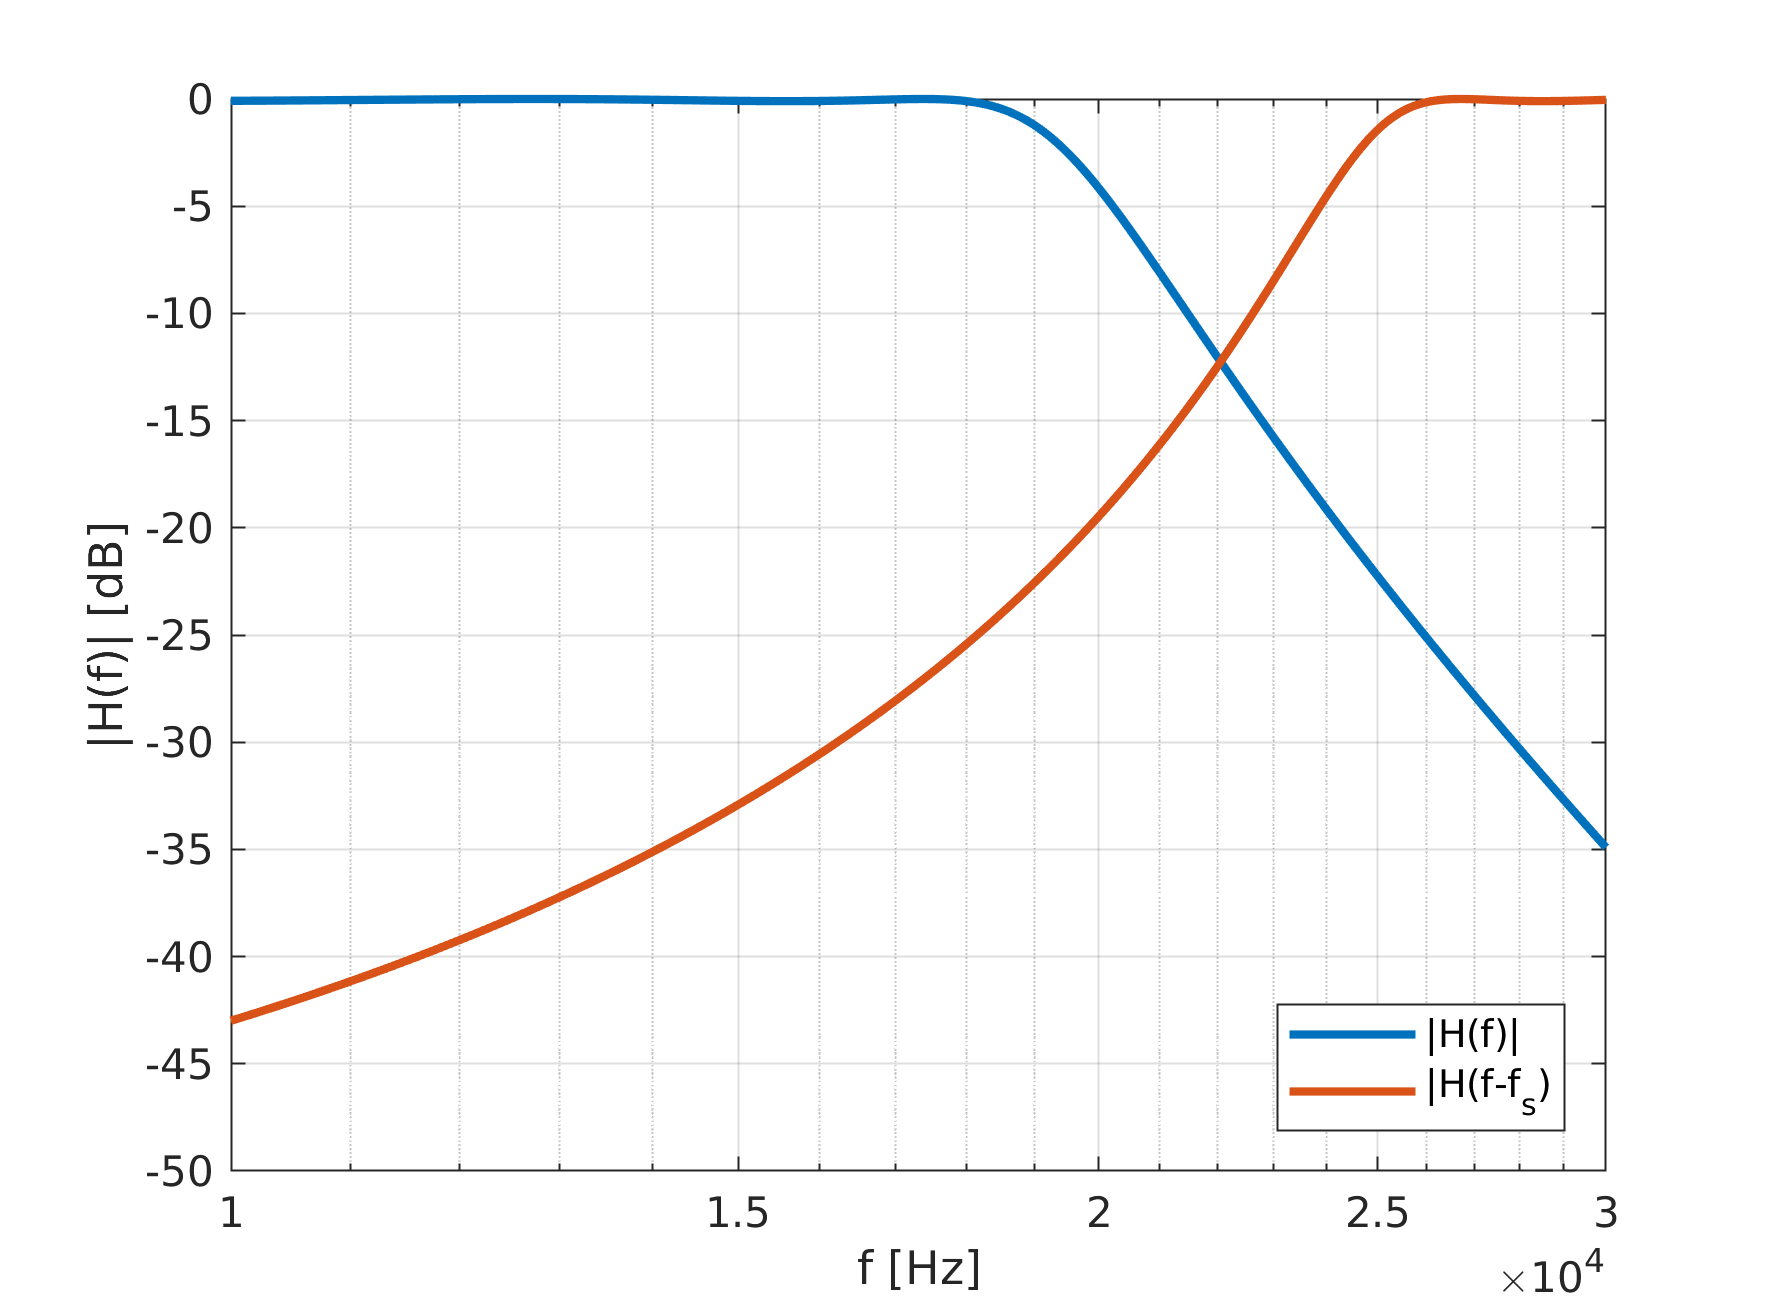
\includegraphics[width=.8\textwidth]{matlab/filter_f_fs.png}
	\caption{}
	\label{fig:filter_f_fs}
\end{figure}

En dæmpning på kun $\num{12.3} \si{\decibel}$ ved Nyquistfrekvensen er ikke ret stor og der må derfor ventes aliasing i signalet.
Størrelsen af aliasing i signalet $SA$, kan beregnes som procentvis del ved
\begin{align}
	\%SA = \frac{|H(f)|_{f=f_s-f_x}}{|H(f)|_{f=f_x}} \cdot 100 \% \label{eq:signal_alias}
\end{align} 
I ligning \ref{eq:signal_alias} angiver $f_x$ den frekvens, hvor den procentvise aliasing effekt ønskes beregnet.
Effekten kan evalueres ved at plotte $SA(f)$ fra ligning \ref{eq:signal_alias} som ses i figur \ref{fig:filter_sa}, både angivet som procentvis forhold og absolut i decibel.
Her er det således muligt at se, at der ved fx $f_c=\num{18}\si{\kilo\hertz}$ er en aliasing effekt på $5,4\%$.

\begin{figure}[h!]
	\centering
	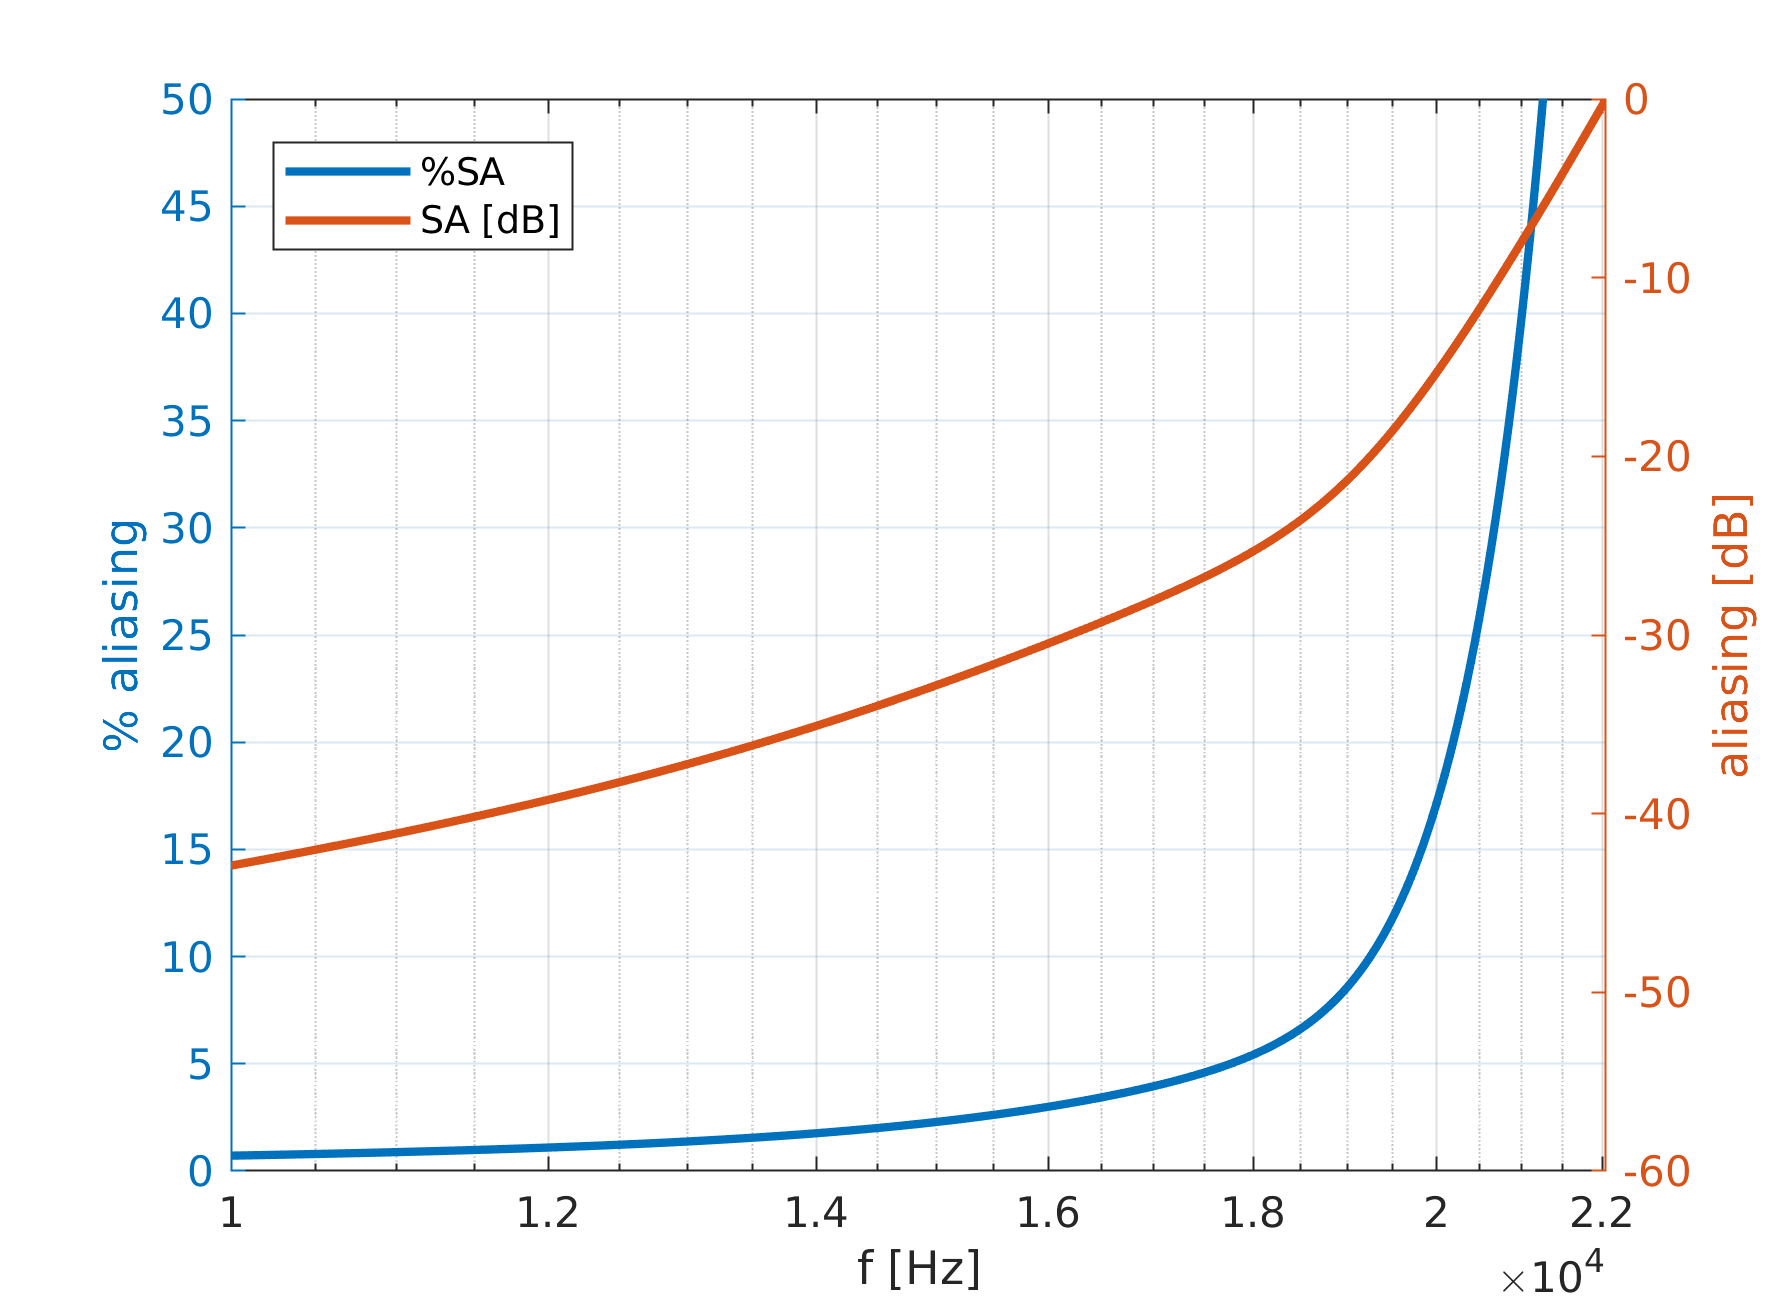
\includegraphics[width=.8\textwidth]{matlab/filter_sa.png}
	\caption{}
	\label{fig:filter_sa}
\end{figure}

%\note{Beregninger og argumentation for SNR}

\section{Specifikation og dimensionering}\label{sec:filter_spec}



\note{sprecifikation som bi-quad systemer}
\note{hvor tæt ligger de beregnede komponent værdier i hold til de anvendte tabelværdier ?}
\note{Sallen Kay - metode 4 i afs matr.}
\note{Hvordan kommer aliasing til at have indflydelse på det endelige signal ved valg af 6. ordens filter} 


\section{Design og implementering}\label{sec:filter_design}
\note{Fremstilling i bi-quad print}
\note{Argumenteret valg er OpAmp -> den bedste der var som SMD}
\note{Kort begrundelse for enkelt R i metoden og brug af op til 4 stk. C som proto type -> hvordan ville det se ud hvis kun brugte den nærmeste C i serien og hvor stor indflydelse vil det have. Måske Sensitivitesmetoden eller H(jw) -> var det er klogt valg og måske lidt overdrevet.}

\section{Rekonstruktions filter}
\note{Hvorfor anvendes et tilsvarende AA filter på udgangen - lidt teori her}


\section{Input stage med pre-amp og DC-offset}
\label{sec:inputstage}
Systemet skal kunne modtage et signal fra en lydkilde, som afspiller lyd i det menneskeligt hørbare område. 
Før signalet kan videreføres til anti aliasing filtrene, skal der være en mulighed for eventuelt at forstærke signalet med en operationsforstærker. 
På den måde kan en fuld opløsning opnås ved den senere AD konvertering. 
\newline
Et almindeligt analogt lydsignal har generelt frekvenser mellem 20Hz og 20kHz, som svarer til det menneskeligt hørbare område. 
Signalets spænding varierer for forskellige kilder. 
Der findes ingen officiel standard, men en del forbruger-elektronik har typisk en maksimal amplitude på 0,447V.\cite{wikiLine} 
\newline
Da signalet skal læses af en "analog to digital converter" som kun kan aflæse spændingsværdier mellem 0V og 3,3V, var det praktisk at anvende en operationsforstærker med 3,3V single-supply.
Dette betyder imidlertid at indggangsignalet der svinger omkring 0V skal påføres et offset således at forstærkeren ikke præsenteres for negative værdier.  
%Til forstærkningen benyttes en aktiv operationsforstærker med 3,3V single-supply. 
%Men indgangssignalet fra lydkilden vil svinge omkring 0V. 
%Derfor skal signalet have et offset, da signalet ellers vil blive klippet hver gang det går under 0V, da operationsforstærkeren ved single-supply ikke har mulighed for at have negative udgangssignaler. 
Det ønskes at indgangssignalet har mulighed for at svinge både så højt og lavt som muligt, så offsettet designes til at være symmetrisk, med respekt til  forsyningsspændingen. 
\begin{equation}
	{V_{offset}} = \frac{V_{supply}}{2} = \frac{3,3\text{V}}{2} = 1,65\text{V}
\end{equation}
Ved et offset på 1,65V kan signalet ideelt have en maksimal amplitude på 1,65V. 
%Herfra skal den valgte operationsforstærkers output swing i forhold til dens forsyningsspænding trækkes fra. (vender tilbage til det her når op-amp skal vælges)
Ved at opbygge en spændingsdeler, kan offsettet skabes. 
Kredsløbet kan ses i bilag \ref{bilag:diagram} under 'Input stages for venstre og højre kanal'.

\subsubsection{Valg af operationsforstærker}
Operationsforstærkeren som skal forstærke signalet vælges ud fra en række krav. 

\begin{itemize}
	\item Forstærkeren skal kunne forsynes med  single-supply 3,3V
	\item Båndbredden skal være minimum 44,1 kHz.
	\item Rail to rail voltage swing skal være så stort som muligt. 
	\item Slew rate skal være hurtig nok til at signalet ikke forvrænges. 
	\item Komponenten skal være tilgængelig som SMD komponent. 
\end{itemize}
Den nødvendige slew rate kan beregnes ved formel \ref{eq:slewrate}.\cite{slewrate}
\begin{equation}
\label{eq:slewrate}
\text{Slew rate} = 2 \pi \cdot f_{maks} \cdot V_{maks} = 2\pi \cdot 22,05\si\kilo\hertz \cdot 1,65\si\volt = 0,23\si[per-mode=symbol]{\volt\per\micro\second}
\end{equation}
Ud fra kravene vælges operationsforstærkeren AD8031 som SMD komponent. 
Forstærkeren kan operere ved en single-supply forsyning ned til 2,7V, har 80MHz -3dB båndbredde ved en forstærkning på 1 og en slew rate på 30\si[per-mode=symbol]{\volt\per\micro\second}
Forstærkerens output swing ligger inden for 20mV af rail-spændingen. Ved 3,3V ligger spændingsvidden således fra 0,02V til 3,28V. 
Forstærkerens specifikationer overgår kravene med en stor margen. 
Det var ikke muligt at finde en anden operationsforstærker som var tilgængelig som SMD, der både havde en acceptabel slew rate, samt muligheden for en single-supply forsyningsspænding på 3,3V. 
Havde der været mere tid, kunne det have været bestilt hjem. 

\subsubsection{Beregning af forstærkning}
For at forstærke signalet, opsættes operationsforstærkeren som en ikke-inverterende forstærker. 
Da indgangssignalets maksimale amplitude vil variere alt efter hvilken kilde det leveres af, skal forstærkningen kunne justeres. 
Derfor sættes en variabel modstand i serie med feedback-modstanden. 
Den valgte variable modstand kan gå fra tilnærmelsesvist at tilsvare en kortslutning og op til 100k$\Omega$.
For at undgå en kortslutning fra operationsforstærkerens output og til den inverterende indgang, er den variable modstand sat i serie med en feedback-modstand på 5k$\Omega$. 
$R_2$ er valgt til 47k$\Omega$, så $R_2$ matcher modstanden fra højpasfilteret. 
I formel \ref{eq:Aminfors} og \ref{eq:Aminfors} ses den mulige maksimum- og minimumsforstærkning.

\begin{equation}
\label{eq:Aminfors}
A_{maks.} = 1 + \frac{R_{feedback} + R_{variabel}}{R_2} = 1 + \frac{5\text{k} \Omega + 100\text{k} \Omega}{47\text{k} \Omega} = 3,23
\end{equation}
\begin{equation}
\label{Amaksfors}
A_{min.} = 1 + \frac{R_{feedback}}{R_2} = 1 + \frac{5\text{k} \Omega}{47\text{k} \Omega} = 1,11
\end{equation}

\subsubsection{Højpas filter-design}
Mellem inputtet og operationsforstærkeren sidder en kondensator, som blokerer DC fra indgangssignalet. 
Som det ses i bilag \ref{bilag:diagram}, vil kondensatoren og modstandene fra offsettet udgøre et højpas filter. 
Filterets knækfrekvens sættes så lavt, at alle frekvenser i det hørbare område ikke påvirkes. 
Ved AC-analyse kortsluttet forsyningen. Derfor sidder modstandene $R1$ og $R2$ parallelt.
%Det endelige kredsløb er kopieret, således der er to udgange for at opnå stereo. 
Stereo blev således opnået ved at anvende to eksemplarer af kredsløbet, en for henholdsvis højre og venstre lydkanal.
\begin{equation}
f_c = \frac{1}{2\pi R C} = \frac{1}{2 \pi \frac{1}{\frac{1}{47k \Omega}+\frac{1}{47k \Omega}}  470\text{nF}} = 14,1\text{Hz}
\end{equation}

\section{Output stage}

%Da de rekonstruerede signal stadigvæk er offset skal DC-værdien fjernes igen inden signalet føres ud af systemet.
Da det rekonstruerede signal stadig har et offset skal DC-værdien fjernes igen inden signalet føres ud af systemet.
Dette gøres ved at anvende en kondensator inden udgangen, dette danner et højpas led med belastningen på udgagen med en knækfrekvens der kan beregnes med ligning \ref{eq:fchp1}.

\begin{equation}
	f_c = \frac{1}{2\pi RC}
\label{eq:fchp1}
\end{equation}

Ved lidt søgning kan der findes frem til at indgangs impedansen på lyd forstærkere og lignende typisk ligger på $10\si{\kilo\ohm}$ og opefter.

Knækfrekvensen skal gerne være på maksimum $20\si{\hertz}$.

Herefter kan ligning \ref{eq:fchp1} omskrives til ligning \ref{eq:fchp2}, for at finde kondensator værdien.

\begin{equation}
	C = \frac{1}{2\pi Rf_c} = \frac{1}{2\pi 10\si{\kilo\ohm} 20\si{\hertz}} = 0,796\si{\micro\farad}
\label{eq:fchp2}
\end{equation}

Det findes så at kondensatoren skal være ca. 0,8\si\micro\farad.
For nemhedens skyld valgtes en værdi på 1\si\micro\farad, da det er en let tilgængeligt standard værdi.
Med denne kondensator vil belastningen kunne være ned til cirka 8\si\kilo\ohm, før at knækfrekvensen vil overstige 20\si\hertz, hvilket overholder kravspecifikationen.






%---------- Chapter ----------------
\chapter{Mikrocontrolleren}\label{kap:mcu}
\vspace*{0.5 cm}
\emph{I det følgende kapitel gives en overordnet gennemgang af de elementer i løsningen der er relateret til mikrokontrolleren. Efter en kort introduktion til FreeRTOS og en oversigt over løsnings taskmodel, følges lydsignalets vej igennem systemet, og derved opnås der en forståelse af systemets enkelte dele. Kapitlet afsluttes med en gennemgang af brugergrænsefladen.}

%---------- Parts ----------------
\section{FreeRTOS}
\note{Kort intro til hvad FreeRTOS er og hvilken funktionalitet det stiller tilrådighed}
Som indlejret styresystem benyttes FreeRTOS. 
FreeRTOS er et open source real-tids styresystem til indlejrede systemer, som er blevet en industriel standard. 
Styresystemet er valgt, da det er simpelt at gå til. 
Det er desuden primært skrevet i programmeringssproget C, som også benyttes i projektet. 
FreeRTOS benytter preemptive schedulering til at administrere CPU-tiden mellem tasks. 

\section{Preemptive schedulering}
FreeRTOS er bygget på en prioritetsbaseret preemptive scheduleringsalgoritme.\newline
Når et operativ system opererer med en preemptive scheduleringsalgoritme kan kørende processer preemptes - blive stoppet - og skiftet ud med en anden proces.\newline
Det kan f.eks. være at en proces der har ventet på en I/O device får tilgang til denne.
Scheduleren vil så skifte den nuværende kørende proces ud og skifte den hidtil ventende proces ind så den kan køres.
Dette gør scheduleren via et context switch.\newline
Når et context switch sker gemmes ''konteksten`` af den nuværende task i en process control block (PCB), og ydermere sker der et state restore, hvor informationen i PCBen af den task, der skal skiftes til hentes.
Det som bliver gemt i PCBen er værdierne i CPU registrene (Program counter, etc.) og anden vigtig operativ systemsinformation.\newline
Prioritetsbaseret skeduleringsalgoritmer tildeler alle tasks en prioritet som er baseret på taskens vigtighed.\newline
FreeRTOS er et real-time operativ system og et primært formål ved real-time operativ systemer er at give et respons på begivenheder indenfor en vis deadline.
FreeRTOS skeduleringsalgoritme sørger så for at den task med højest prioritet bliver givet processortid.

\note{afsnit om task, task model, hid queues og implementering i os}

\section{Interrupt håndtering}
\note{Interrupt execution diagram og opsætning} 
\subsection{Intterrupt eksekvering og task skedulering}
Figur \ref{fig:int_task} viser hvordan tasks og interrupts håndteres i FreeRTOS. 
Til tiden t1 kører en lavt prioriteret task. 
Ved t2 bliver en interrupt service rutine, fremover kaldet en ISR, kaldt. 
Den prioriteres højest, og den lavt prioriteret task pauses indtil ISR'en er færdig.
ISR'eren er færdig til tiden t3, hvor den lavt prioriteret task kan genoptages.
Ved t4 sker et context switch til en højere prioriteret task.
Skeduleringen mellem tasks er styret af FreeRTOS scheduler med respekt til den prioritet, som hver task er givet. 
Interrupts prioriteres højere end alle tasks, uanset prioriteten af den pågældende task. 
Interrupts har også prioriteter i mellem sig, såfremt flere skulle blive kaldt. 
Modsat tasks, vil en interrupt dog altid afsluttes, før den næste kan begynde. 
ARM Cortex-M4 tilbyder otte interrupt prioriteter. 
\husk{Jes}{Forstået rigtigt?} 
\begin{figure}[h]
	\caption{Det tidslige forløb for to tasks og en interrupt service rutine. }
	\centering
	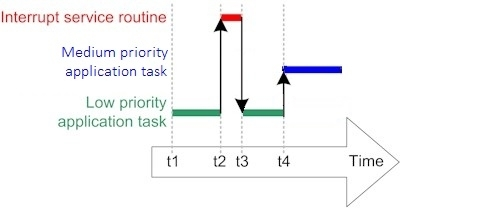
\includegraphics[width=0.6\linewidth]{billeder/interruptandtaskprocessing.jpg}
	\label{fig:int_task}
\end{figure}

Når det indgående lydsignal skal samples gennem ADC'en, skal samplingen foregå periodisk på nøjagtigt det samme tidspunkt i hver periode.
Det faste tidspunkt for sampling giver minimal jitter med en minimal forsinkelse i samplingen af signalet. 
\husk{Jes}{Dansk ord for jitter? Det er et teknisk engelsk ord, så det kan vel gå.. } 
For at sikre, at mikrocontrolleren sætter alle andre opgaver på pause, og begynder at sample på det korrekte tidspunkt, implementeres samplingen i en ISR.

\subsection{Implementering af interrupt-styring med timer}
ISR'en indstilles med den højest mulige interrupt prioritet. 
Timingen af ISR'en er styret af Timer 3. 
Timeren er implementeret som en 16-bit timer i periodic timer mode, edge-count mode og inverted PWM mode.
Ved start hentes timerens start value ind i et tælleregister. 
Sample-frekvensen og CPU frekvensen styrer værdien. 
\begin{equation}
	\text{Timer start value register} = \frac{\text{CPU'ens frekvens}}{\text{Sample-frekvens}} = \frac{80\text{MHz}}{44,1\text{kHz}} \simeq 1814
\end{equation}
I periodic timer mode vil timeren dekrementere fra tælleregisteret, som automatisk henter timer start værdien igen, og begynder forfra når værdien når nul. 
Når værdien når nul, kaldes den ISR som sikrer at lydsignalet bliver samplet. \newline

\section{Sampling af lydsignal igennem ADC}
Microcontrolleren har to identiske ADC moduler, som opererer uafhængigt ad hinanden. 
De kan derfor sample på samme tidspunkt. 
ADC'erne er opbygget med Successive Approximation Register arkitektur, som leverer en opløsning på 12-bit, hvilket giver 4096 mulige steps i det digitale resultat. 
ADC'ens interne forsyningsspænding og ground er på henholdsvis 3,3V og 0V, hvilket samtidig er den maksimale og minimale spændingsreference, som ADC'en kan læse. 
Stepsizen er $\Delta$ er udregnet i formel \ref{eq:ADC_res}.
\begin{equation}
\label{eq:ADC_res}
	\Delta = \frac{X_{maks}-X_{min}}{steps} = \frac{3\text{V}-0\text{V}}{4096} = 0,73\text{mV}
\end{equation}
\husk{Jes}{Stepsize udregning kan måske udelades, hvis vi får pladsmangel.}
ADC'en er drevet af en 16MHz clock, og det tager 250ns at tage én sample. 

\subsection{Opsætning og virkemåde af ADC}
ADC0 og ADC1 er sat op til at modtage et analogt signal direkte på to general purpose input pins (GPIO). 
Start af sampling er indstillet, så det trigges af et processor event. 
Det betyder at en sampling påbegyndes 

Sampling trigges som et procesor event. 

Sample sequencers modtager resultatet. 

% Sample specifikationer
% Valg
	% to stk
	% tid per sample. Hvad kan nås osv. 
	% opløsning
	% Float og offset justering

\section{Modulær opbygning af effekter}

\subsection{Generering af PWM-signal til DAC}
Timeren benyttes desuden til at generere et PWM-signal, hvis duty cycle er styret af timeren og resultatet af A/D konverteringen af indgangssignalet. 
\begin{wrapfigure}{r}{0.5\textwidth}
	\centering
	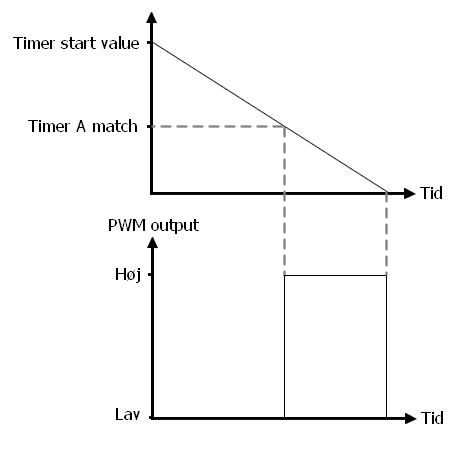
\includegraphics[width=0.5\textwidth]{billeder/timer3PWM.png}
	\caption{\label{fig:PWMfromtimer}Generering af PWM-signal ud fra timer. }
\end{wrapfigure}
Figur \ref{fig:PWMfromtimer} viser hvordan PWM-signalets duty cycle bliver bestemt af den værdi, som bliver gemt på Timer A's match register. 
Den værdi kommer fra den periodiske sampling af lydsignalet gennem ADC'en, hvor resultatet af hver sampling netop gemmes i match registeret. 
Således genskabes signalet som et digitalt PWM signal. 

\section{Genskabelse af signal via DAC igennem SPI}

\section{Håndtering af brugergrænseflade og human input interface}

\husk{Sonny}{Kan dette anvendes?}
For at kunne anvende enheden skal enheden kunne udveksle nødvendige informationer med brugeren, input skal altså kunne modtages, her valgte gruppen at anvende en "drehimpulsgeber", og respons skal oplyses, her valgte gruppen et grafisk repræsenteret menu system.
En menu består en række valgmuligheder repræsenteret af elementer brugeren kan bladre igennem og vælge imellem.
Et valg kan lede til yderligere valgmuligheder inden for den valgte kategori, disse kan så præsenteres i form af en ny menu.
Til at udføre denne funktion valgte gruppen at anvende linkede lister.
I eksemplet herunder ses en hovedmenu "Root Menu" som linker til sit første element "Master volume", vælger brugeren dette element kan volumen sættes, elementet linker også til næste element så brugeren kan skifte til det, her er der tale om "Echo" elementet som istedet for at have en funktion linker til en ny menu nemlig "Echo menu" som så linker til sin egen liste af menu punkter.
En "drehimpulsgeber" kan anvendes til at producere 3 forskellige typer af input, drej mod uret herefter kaldet "vr", drej med uret "hr" og click.
Når et input  modtages af programmet lægges det i en input kø til systemet er klar til at modtage input, er der tale om et "vr" fremvises foregående element i menuen, på samme måde anvendes et "hr" input til at gå til næste element i menuen og et click anvendes til at vælge det det nuværende element.


%---------- Chapter ----------------
\chapter{Effektmoduler}\label{chap:DSP}

\section{Echo effektmodul}\label{sec:echo}
\note{ved ikke om det skal ligge her}
Et echo opstår når en lydbølge reflekteres tilbage på en overflade, sålede at den kan høres igen blot forsinket den tid, det tager for lyden at bevæge sig gennem luften.
Det vil sige at jo længere væk overfladen, som lyden reflekteres på, er fra udgangspunktet for lydkilden og hvor lyden høres, jo længere går der imellem den oprindelige lyd og echoet.
Et echo opstår som regel i et stort åbent område hvor der så er en eller flere store relativt ubrudte flader, såsom facaden på en stor bygning eller en bjergside.
Også i nogle tunneler der har den rigtige udformning kan der opnås en god echo effekt.
Ved et echo reflekteres lydbølgen oftest tilbage til kilden relativt få gange og gerne med en lidt stor forsinkelse.

\section{Implementering af echo effektmodul}
Vi ønsker at implementere en echo effekt der virker real time på microcontrolleren , således at der kan føres et lydsignal ind, og der med det samme kommer et modificeret lydsignal ud.
Dette gøres ved at gemme en dæmpet kopi af outputsignalet i en buffer og efter en valgt forsinkelse, i form af et bestemt antal samples, bliver dette gemte signal lagt til udgangsignalet og igen bliver en kopi af dette gemt,således at der dannes et feedbackloop som det ses på figur (\ref{fig:echo_simulink}).
\note{Her beskrives ikke rigtigt hvordan bufferen virker, dette beskrives dog nede i reverb delen derfor tænker hjeg måske at echo skal flyttes?}
\begin{figure}[h]
	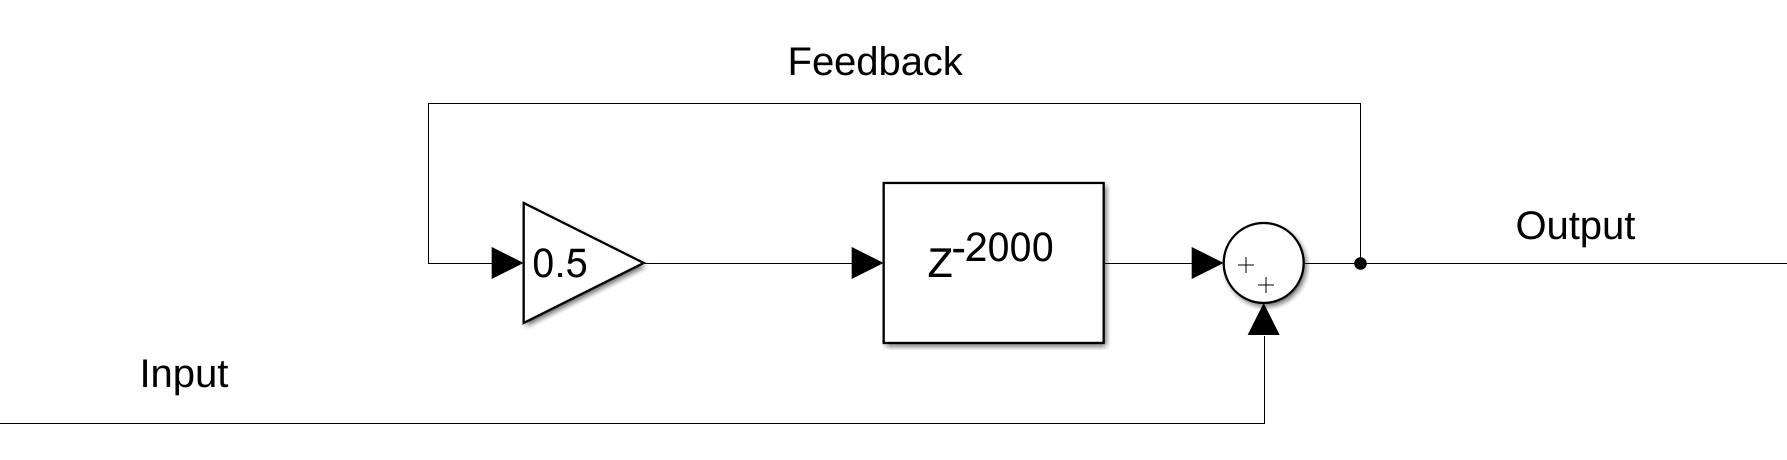
\includegraphics[width=0.8\linewidth]{./billeder/Echo_simulink.png}
	\caption{Simulink model af echo effekt.}
	\label{fig:echo_simulink}
\end{figure}

\section{Reverb effektmodul}\label{sec:reverb}
Reverb, rumklang, er resultatet af lydbølger som bliver reflekteret tilbage af %samtlige overflader med forskellige vinkler.\newline
%Rumklang er resultatet af lydbølger som bliver reflekteret af samtlige overflader i et rum, derved bygges der en masse reflektioner op hvis amplitude falder mod $0$ som de bliver absorberet af overfladerne i rummet.\newline
overfladerne i et givent lokale, dette påvirker lyden ud fra tre kriterier.\newline 
Et overfladerne kan bestå af forskellige materialer som afgør hvor stor en del af lydbølgen der reflekteres.\newline 
To afstanden mellem en given overflade, lydkilden og modtageren kan variere, dette giver reflektioner med forskellig forsinkelse samt forskellige amplituder da lydbølgen aftager i styrke jo længere den bevæger sig.\newline 
Tre overfladerne kan have forskellige vinkler som kan lede til at lydbølger reflekteres mellem en række overflader før de når modtageren, dette resultere i en kaskade af de effekter de andre to kriterier har.\newline
Der er to primære metoder for implementeringen af en digital reverb effekt convolution reverb og den algoritmisk reverb.
\subsection{Convolution reverb}
Reverberation, rumklang, er en tidsinvariant effekt, hvilket betyder at det ikke har nogen betydning, hvornår en tone bliver spillet, det vil ultimativt resultere i præcis den samme reverberation. \newline
Tidsinvariante systemer kan karakteriseres ved deres impulsrespons.
Et convolution reverb virker ved at lave en matematisk foldning af det ønskede %rummets 
impulsrespons og det lydsignal der skal tilføres en rumklang.\newline 
% sættes på indgange til reverben.\newline

%Dette skaber en realistisk rumklangseffekt, fordi impulsen i dette tilfælde vil være en lyd som holder samme energiniveau ved alle frekvenser.
En realistisk rumklangeffekt kan opnås ved at optage og anvende impulsresponsen fra et rum med den ønskede rumklang.
Dette gøres ved at producere en lyd impuls, et kort brag, eksempelvis ved at springe en ballon, og så optage den resulterende lyd. 
%Efter impulsen bliver spillet vil den blive reflekteret rundt i rummet.
%Nogle af reflektionerne møder mikrofonen med det samme mens andre bliver ført rundt i rummet og amplituden af signalerne går mod $0$ pga. overfladerne af objekterne i rummet absorbere energien fra dem.\newline
%Multiplikering af hver punkt af impulsresponset med amplituden af samplet giver så rummets respons til den sample.
Ved at multiplicere hvert punkt af impulsresponset med amplituden af en sample fås så rummets respons til den sample.
%Dette gøres for hver sample af inputtet og giver overlappende responser som så adderes og resulterer i rumklang.
%En ulempe ved convolution reverbs er, at der skal mange beregninger til for at få resultatet.
De primære ulemper ved convolution reverb metoden er at der skal mange beregninger til for at få resultatet og at der skal anvendes en del hukommelse til at gemme impulsresponset fra rummet med en ønskede klang.
Da hver sample individuelt skal multipliceres med hver sample af impulsresponset og adderes til outputtet med den passende forsinkelse i tid, kan antallet af beregninger findes ved $N \cdot M$, hvor $N$ er antallet af samples impulsresponset fylder, altså samplings frekvensen multipliceret med længden af impulsresponset, og $M$ er samplings frekvensen.
Har man eksempelvis bruger et impulsrespons på $1$ sekund optaget ved $44.1\si{kHz}$ til at tilføje en rumklang til et stykke lyd der også bliver samplet ved $44.1\si{kHz}$, får man at det er nødvendigt med $1944810000$ multiplikations og additions  operationer i sekundet, altså lige knap $2$ milliarder operationer i sekundet. 
%Hvis der haves $N$ samples og impulsresponset er $M$ samples lang skal der udføres $N+M$ multiplikationer og additioner.
%F.eks. hvis der haves et impulsrespons på 1 sekund og der samples med $44.1\si{kHz}$, skal der udføres næsten 2 milliarder multiplikationer og additioner i sekundet.
%Antallet af multiplikationer og additioner kan dog reduceres drastisk ved at arbejde i frekvensdomænet i stedet for, da foldning i frekvensdomænet er multiplikation.

Fordelen ved convolution reverbs er at ethvert rum i verden kan imiteres, hvis impulsresponset for det valgte rum haves.\newline
Derudover kan man opfinde rum ved at syntetisere et impulsrespons.

\subsection{Algoritmisk reverb}
En algoritmisk reverb virker ved at bruge flere forskellige delays med tilhørende gains der sænker signalets styrke og feedback loops til at opbygge en serie af ekkoer, som dør ud over tid.
Det er sammensætningen af de basale byggeblokke som giver karakteristikken på rummet der emuleres.\newline
Et eksempel på en simpel algoritmisk reverb effekt er all-pass filteret.
%insert billede af all-pass filter
\begin{figure}[h]
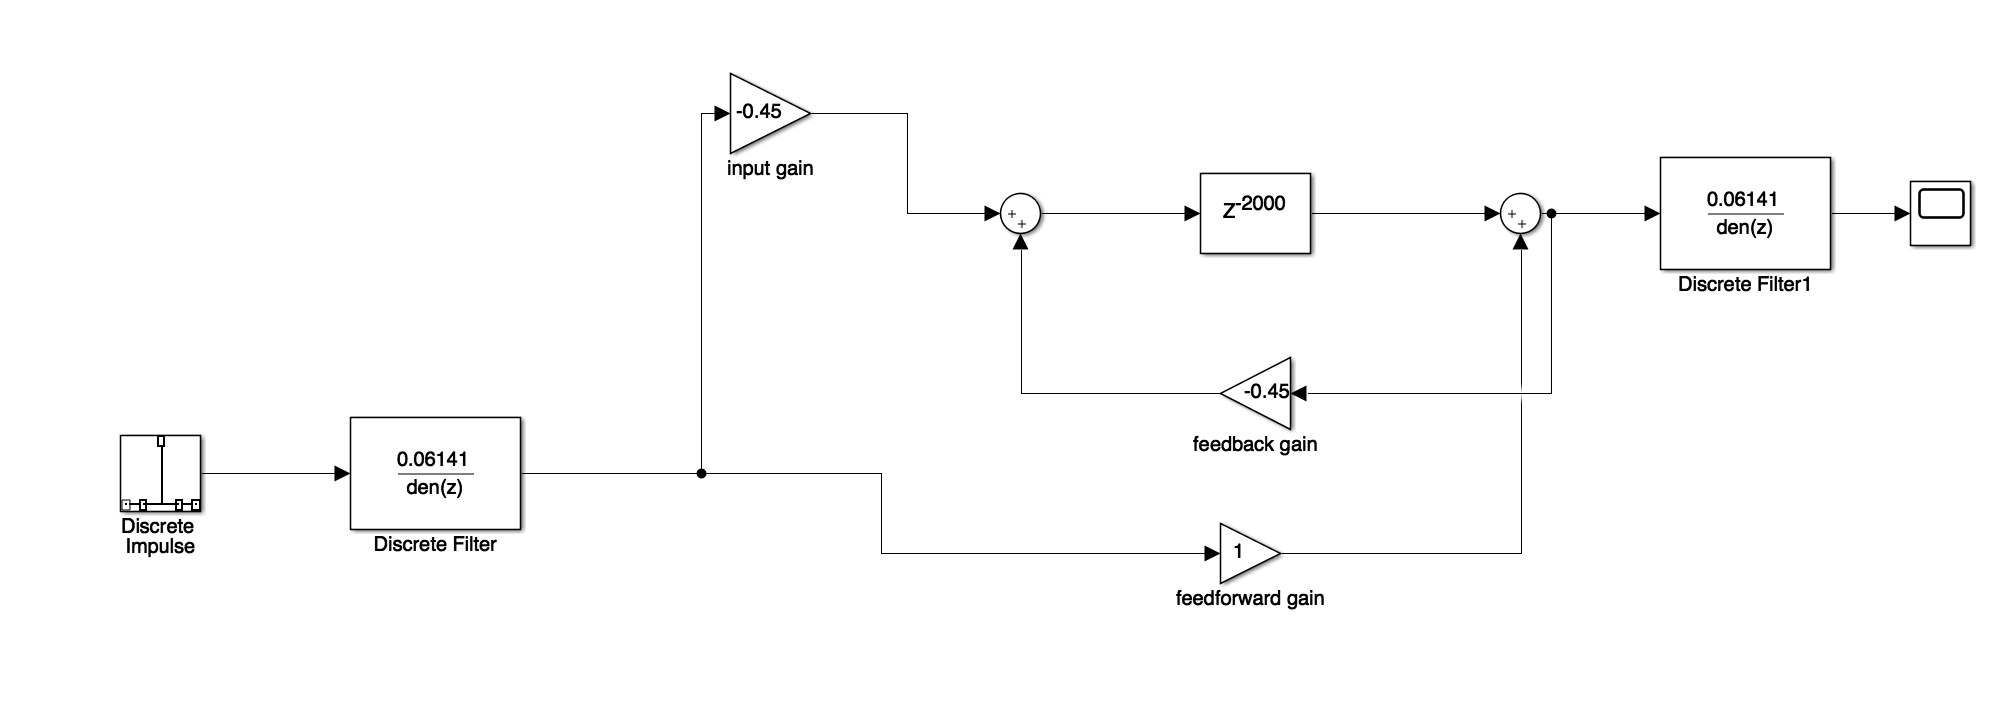
\includegraphics[width=0.8\linewidth]{./billeder/reverb-testopsaetning.png}
\caption{All-pass reverb filter i matlab.}
\label{fig:allPassMatLab}
\end{figure}
Her bliver en sample feeded forward til outputtet så lyden bliver spillet med det samme.
Derudover gemmes den i en reduceret og inverteret udgave. %smides samplet ind i en delay buffer.
%Rumklangen skabes så af samples fra delay bufferen, som fungerer som opbygningen af ekkoer og feedback loopet som agerer som absorptionen for at skabe aftagende ekkoer.
Rumklangen der skal tilføres til tiden fastsat af en delay tid kan så fremstilles af de gemte samples samt en brøkdel af outputtet.
Resultatet gemmes og bliver tillagt outputet til delay tiden og dermed opnås en række aftagende ekkoer.
Ulempen ved denne metode er at den skal serie kobles flere gange med forskellige delay tider for at opnå realistiske resultater.




\section{Implementering af reverb}
Gruppen valgte at implementere en algoritmisk reverb funktion da mikrochippen tilrådighed kun havde en meget begrænset mængde hukommelse.
Dette blev opnået ved at anvende en buffer til konstant at gemme reducerede samples af input og output som så kunne tilføjes outputtet til delay tiden.

Bufferen der blev valgt at implementere til dette er af en cyklisk natur, hvor der til hver samplingstid udlæses en værdi fra den af pointeren indikerede plads, pladsen nulstilles så og pointeren incrementeres så der til næste sample udlæses fra den næste plads i bufferen, herved opnås en buffer hvor der kan indsættes værdier der skal tilføres outputtet med en given forsinkelse angivet i antal samplingstider senere. 



\section{FIR filter}
Som et effektmodul blev der udviklet et FIR (finite impulse response) filter, hvilket vil sige at impulsresponset af filteret falder til nul efter et vist stykke tid.\newline
Et FIR filters overføringsfunktion er givet ved
\begin{equation}
H(z) = b_0 + b_1z^{-1} + \cdots + b_Kz^{-K}
\end{equation}
Hvori $b_i$ er filterets koefficienter.\cite[p.218]{Tan2013}\newline
Filteret og dets koefficienter bliver ved run-time beregnet efter brugeren inputter cutoff frekvensen. Filteret designes og det koefficienter bliver beregnet via frequency sampling metoden.
Grunden til frequency sampling valgtes som designmetode er, fordi algoritmen er baseret på invers diskret frekvens/tid fourier transformation (IDFT), hvilket kan beregnes effektivt via FFT.\newline
\subsection{Frequency Sampling}
Frequency sampling metoden virker ved at man lader $h(n)$ for $n = 0, 1, \cdots, N - 1$ approksimere filterets impulsrespons, hvor $N$ er antal koefficienter, hvilket for FIR filtre er deres koefficienter, og $H(k)$ for $k = 0, 1, \cdots, N - 1$ er de diskrete Fourier transformationskoefficienter.
\begin{figure}[!ht]
	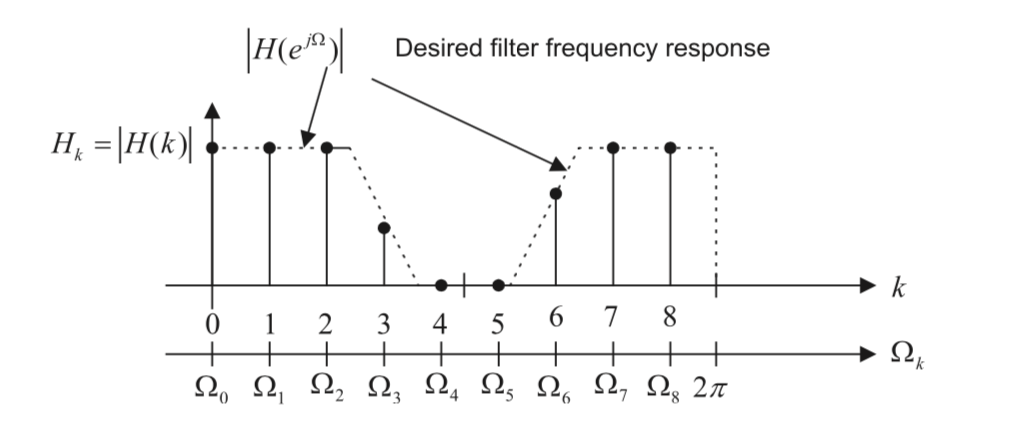
\includegraphics[width=\textwidth]{billeder/frequencysampling.png}
	\caption{Frekvenssampling af amplitudekarakteristik\cite{Tan2013}}
	\label{fig:frequencysampling}
\end{figure}
$H(k)$ findes ved at sample den ønskede amplitudekarakteristik i frekvensdomænet ved lige adskilte frekvenser som vist i figur (\ref{fig:frequencysampling}).\newline
FIR koefficienterne findes så ved
\begin{equation} \label{eq:fir_koefficienter}
b_n = h(n) = \frac{1}{2M + 1} \left\{H_0 + 2\displaystyle\sum_{k = 1}^{M}\, H_k\cos\left(\frac{2\pi k (n - M)}{2M + 1} \right) \right\} \quad \mathrm{for} \quad n = 0, 1, \cdots, M
\end{equation}
hvor $M = \frac{N - 1}{2}$
Resten af koefficienterne findes ved $h(n) = h(2M - n) \quad \mathrm{for} \quad n = M + 1, \cdots, 2M$ ved brug af symmetri, når filteret antages at have lineær fase.


\subsection{Implementering af FIR filter}
Det digitale filter blev valgt at blive implementeret som et FIR filter, fordi FIR filtre giver mulighed for at have lineær negativ fase hvilket medfører konstant gruppeløbetid.\newline
Negativ lineær fase medfører konstant gruppeløbetid da gruppeløbetid er givet ved
\[
\tau = -\frac{\mathrm{d}\varphi}{\mathrm{d}\omega}
\]
Konstant gruppeløbetid er en fordel at have i audio applikationer da en varierende gruppeløbetid kan komme til at lyde forkert.\newline
Modulet virker ved at det tager en cutoff frekvens som brugerinput og dernæst beregner normerede cutoff frekvens ved
\[ \Omega_c = 2\pi\frac{f_c}{f_s} \]
Hvor $f_c$ er cutoff frekvensen og $f_s$ er samplingsfrekvensen.
Dernæst beregnes en array af amplitudekarakteristikken $H_k$ for de normerede frekvenser fra $0$ til $\pi$ ved 
\[ \Omega_k = \frac{2\pi k}{(2M + 1)} \quad \mathrm{for} \quad k = 0, 1, \cdots, M \]
Når $H_k$ haves beregnes $M$ filterkoefficienter via. ligning (\ref{eq:fir_koefficienter}) og resten findes ved symmetri.\newline
Filteret virker ved at en buffer fyldes med $x$ samples og dernæst bliver der foretaget en foldning for hver sampel i bufferen med hver filterkoefficient.

%\section{Delkonklusion}
\section{Opsummering}
En betydelig begrænsning i implementering af effektmodulerne er den korte tid mellem at en samples modtages og sendes ud igen.
Dette betyder at  meget store og eller komplicerede beregninger simpelthen ikke kan udføres hurtigt nok til at undgå forsinkelser der kan opfattes af det menneskelige øre.
Det er derfor vigtigt at optimere og begrænse alle beregninger så de bruger den mindste tid muligt. 
Echoeffekten blev implementeret algoritmisk via en delay buffer hvor der gemmes en dæmpet del af inputtet.
Ved brug af samme delay buffer blev reverbeffekten implementeret algoritmisk som et all-pass filter, dette er udført ved at anvende samme metode som echoeffekten samt et feedback loop hvor en dæmpet udgave af outputtet også bliver tilføjet delay bufferen.
%Ved både Echo- og Reverbeffektmodulerne er dette tilfældet, da der ved hvert sample kun skal laves et ganske lille antal simple beregninger.
%I Echoeffektmodulet er bliver et sample blot ganget med en gain/decay \note{hvad kalder vi det?} og derefter adderet til en værdig i en buffer.
%Reverbeffekten opnås ved en lignende metode, det er næmlig valgt at benytte en algoritmisk reverb frem for convolution reverb, altså ved foldning.
Dette er valgt, selvom der i teorien ville kunne opnås en bedre, mere realistisk, reverbeffekt ved convolution reverb.
Valget er truffet, da det ville betyde at der skulle foretages flere beregninger imellem input og output samples.
Hvilket ville betyde, at der ville være en risiko for ikke at nå beregningerne, uden en stor mængde planlægning af beregningerne.
Denne metode har også behov for en større mængde hukommelse end den algoritmiske reverb effekt.
Dette er også en af grundende til, at dette valg blev truffet. 
Da det endte med en pladsmangel på microcontrolleren, når der skal ligge flere forskellige moduler på.
%Echoeffekten blev implementeret algoritmisk via en delay buffer og et feedback loop således at inputtet bliver ført tilbage med en dæmpning på.\newline
%Reverbeffekten blev implementeret som et all-pass filter, hvorved samples bliver ført ind i et dæmpningsled samt en delaybuffer samt at blive outputtet med det samme.
Filtereffekten blev implementeret som et FIR filter da disse giver mulighed for negativ lineær fase som medfører konstant gruppetid.
Der blev valgt frequency sampling som design metode, da den giver fine resultater og fordi algoritmen kræver relativt få beregninger, hvilket gør den godt egnet til real-time filter design.





%---------- Chapter ----------------
\chapter{Diskussion og vurdering}\label{kap:diskussion}
\vspace*{.5cm}


%MCU


%DSP
En betydeligt mere realistisk rumklangs/ekko effekt kunne have været opnået med et ''convolution reverb``, dette ville dog have krævet en bedre microcontroller med højere clock og mere plads til at gemme data og der blev derfor i stedet valgt at anvende algoritmiske løsninger.

%En af de begrænsende faktorer ved implementering af effektmodulerne er den korte tid, der er til at foretage beregninger mellem samples bliver taget til de skal ud igen.
%Den begrensede tid kan skabe et problem for store beregninger der kan tage lang tid, hvis en sådan beregning på signalet ikke bliver færdiggjort før samplet skal ud igen bliver signalbehandlingen ikke korrekt udført, eller det kan resultere i et delay af signalet, hvilket ikke ønskes. \husk{Emil}{jeg her helt bestemt ikke tilfreds med denne sætning...}
%Af hensyn til dette er det vigtigt at lave beregninger så hurgtigt og effiktivt som muligt.

%En betydelig begrænsning i implementering af effektmodulerne er den korte tid mellem at en samples modtages og sendes ud igen.
%Dette betyder at  meget store og eller komplicerede beregninger simpelthen ikke kan udføres hurtigt nok til at undgå forsinkelser der kan opfattes af det menneskelige øre.
%Det er derfor vigtigt at optimere og begrænse alle beregninger så de bruger den mindste tid muligt. 
%\husk{Sonny}{Har skrevet en alternativ udgave af teksten herover}
%Ved både Echo- og Reverbeffektmodulerne er dette tilfældet, da der ved hvert sample kun skal laves et ganske lille antal simple beregninger.
%I Echoeffektmodulet er bliver et sample blot ganget med en gain/decay \note{hvad kalder vi det?} og derefter adderet til en værdig i en buffer.
%Reverbeffekten opnås ved en lignende metode, det er næmlig valgt at benytte en algoritmisk reverb frem for convolution reverb, altså ved foldning.
%Dette er valgt, selvom der i teorien ville kunne opnås en bedre, mere realistisk, reverbeffekt ved convolution reverb.
%Valget er truffet, da det ville betyde at der skulle foretages flere beregninger imellem input og output samples.
%Hvilket ville betyde, at der ville være en risiko for ikke at nå beregningerne, uden en stor mængde planlægning af beregningerne.
%Denne metode har også behov for en større mængde hukommelse end den algoritmiske reverb effekt.
%Dette er også en af grundende til, at dette valg blev truffet. 
%Da det endte med en pladsmangel på microcontrolleren, når der skal ligge flere forskellige moduler på.

	
						
%---------- Chapter ----------------
\chapter{Konklusion} \label{kap:konklusion}

							


\SingleSpacing

\nocite{*}
\bibliography{rapport}\label{bilag:litteratur}
%\listoffigures
%\listoftables

%--------- Bilag -------------------
\appendix
%\chapter{Bilag}
\section{Test af det samlede system}
\label{kap:test}
Testens formål er at udføre en vector network analyse af det samlede system for at finde systemets amplitude-karakteristik. 
Det samlede system består af modtageren af indgangssignalet, anti-aliasing filtrene for den ene kanal, Tiva-kittet med EMP board og microcontroller, DAC, rekonstruktionsfilteret for den ene kanal og udgangskredsløbet. 

\subsection{Udstyr}
\begin{itemize}
	\item Bode 100 med tilhørende udstyr
	\item Èn computer med Bode Analyzer Suite installeret
	\item To oscilloskop-prober
	\item Skillekondensator
\end{itemize}

\subsection{Fremgangsmåde og forsøgsopstilling}
Opsæt Bode 100 uden noget tilsluttet. 
Åben Bode Analyzer Suite, og vælg en Gain/Phase-analyse under Vector Network Analysis. 
Analysen sættes op med følgende indstillinger:
\begin{multicols}{2}
\begin{itemize}
	\item Startfrekvens: 10 Hz
	\item Slutfrekvens: 50 kHz
	\item Minimum 401 data points
	\item Source level: 0 dBm
	\item Attenuator på receiver 1 \& 2: 10 dB
	\item Receiver bandwidth: 100 Hz
	\item External reference på CH1 \& CH2
\end{itemize}
\end{multicols}
Vælg Trace 1 til Magnitude (dB). \newline
Med Bode Analyzer suite laves en kalibrering af Bode 100, når udgangen og indgangene på Bode 100 er koblet sammen. 
Skillekondensatoren skal være på udgangen. \newline
Opsæt det samlede system som vist på figur \ref{fig:lol}. 
Bode 100's udgang med skillekondensator og CH1 kobles til indgangen på den ene kanal af det samlede system. 
CH2 kobles til udgangen af det samlede system for den tilsvarende kanal. 
Analysen kan nu udføres. 

\subsection{Resultat af test}
Datasættet for resultatet af testen kan ses i den vedhæftede fil \textit{'habibi.csv'}. 
\husk{Jes}{Filnavn skal rettes her!}
\begin{figure}[h]
	\caption{Overføringsfunktionen af det samlede system.}
	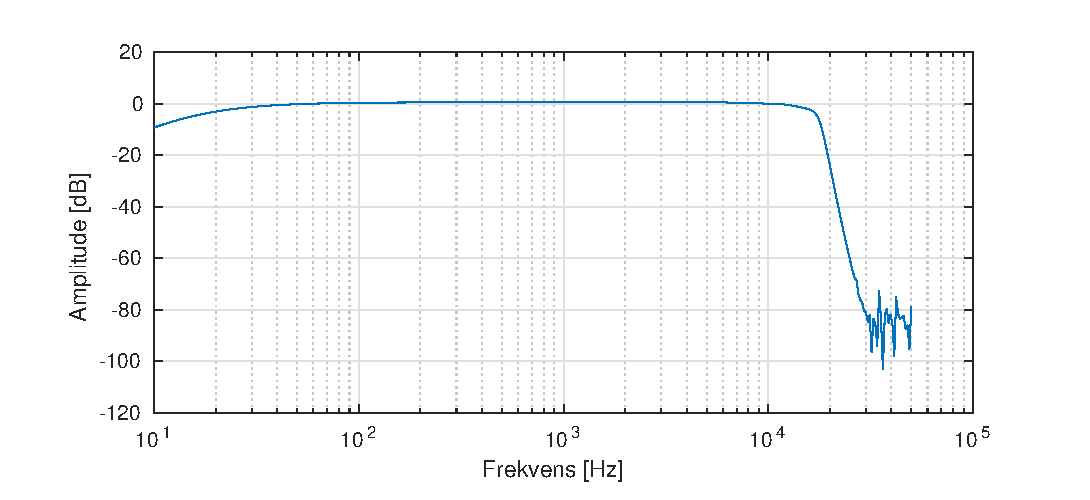
\includegraphics[width=1\linewidth]{./billeder/tf_samletsystem.eps}
	\label{fig:tf_samletsystem}
\end{figure}

\section{Test af anti-aliasing filtre}
%Formål her.
Testen følger samme fremgangsmåde, som ved testen af det samlede system. 
Dog testes udelukkende anti-aliasing filtrene.  
\chapter{Test af reverb og echo impulsrespons}\label{sec:test_af_effekt}
Da echo og reverb begge er tidsinvariante effekter betyder det, at de kan karakteriseres af deres impulsrespons.\newline
Testens formål er at finde impulsresponset for echo- og reverbeffekten.
%Systemet består af modtager af indgangssignal, anti-aliasing filtre, TIVA-kit med EMP board, DAC, rekonstruktionsfilter og udgangskredsløbet.
Systemet består af et signalindgangs board, en række anti-aliasing og input filtre, et TIVA-kit med EMP board, et board med en DAC, nogle rekonstruktionsfilter og et udgangskredsløbet.
\section{Forsøgsopstilling og fremgangsmetode}
\begin{itemize}
	\item Funktionsgenerator sat på pulse med en peak-to-peak spænding sat til $500\si{mV}$ og et DC-offset sat til $250\si{mV}$ og pulsen sættes til at være $25\si{\mu S}$ lang svarende til en sample
	\item Oscilloskop sat til single sweep med en trigger sat til $200\si{mV}$
	\item Load modstand koblet på udgangen på $10\si{k\Omega}$
	\item Reverb delay sat til $10\si{mS}$ og input- og feedbackgain sat til $-0.50$
	\item Echo delay sat til $44\si{mS}$ samples og gain sat til $0.5$
\end{itemize}
%Funktionsgeneratoren kobles på signalindgangen af systemet, og oscilloskopets prober placeres hhv. på indgangen til mikrocontrolleren og på udgangen af rekonstruktionsfilteret.\newline
Funktionsgeneratoren kobles på signalindgangen sammen med en af oscilloskopets prober, den anden placeres udgangskredsløbet.\newline
Effektmodulerne aktiveres hver for sig og der tages et single sweep.
\subsection{Resultat}
Inputtet er den første impuls angivet som den gule graf og outputtet er vist ved den røde graf:
\begin{figure}[!ht]
		\centering
	\begin{minipage}{0.50\textwidth}
		\centering
		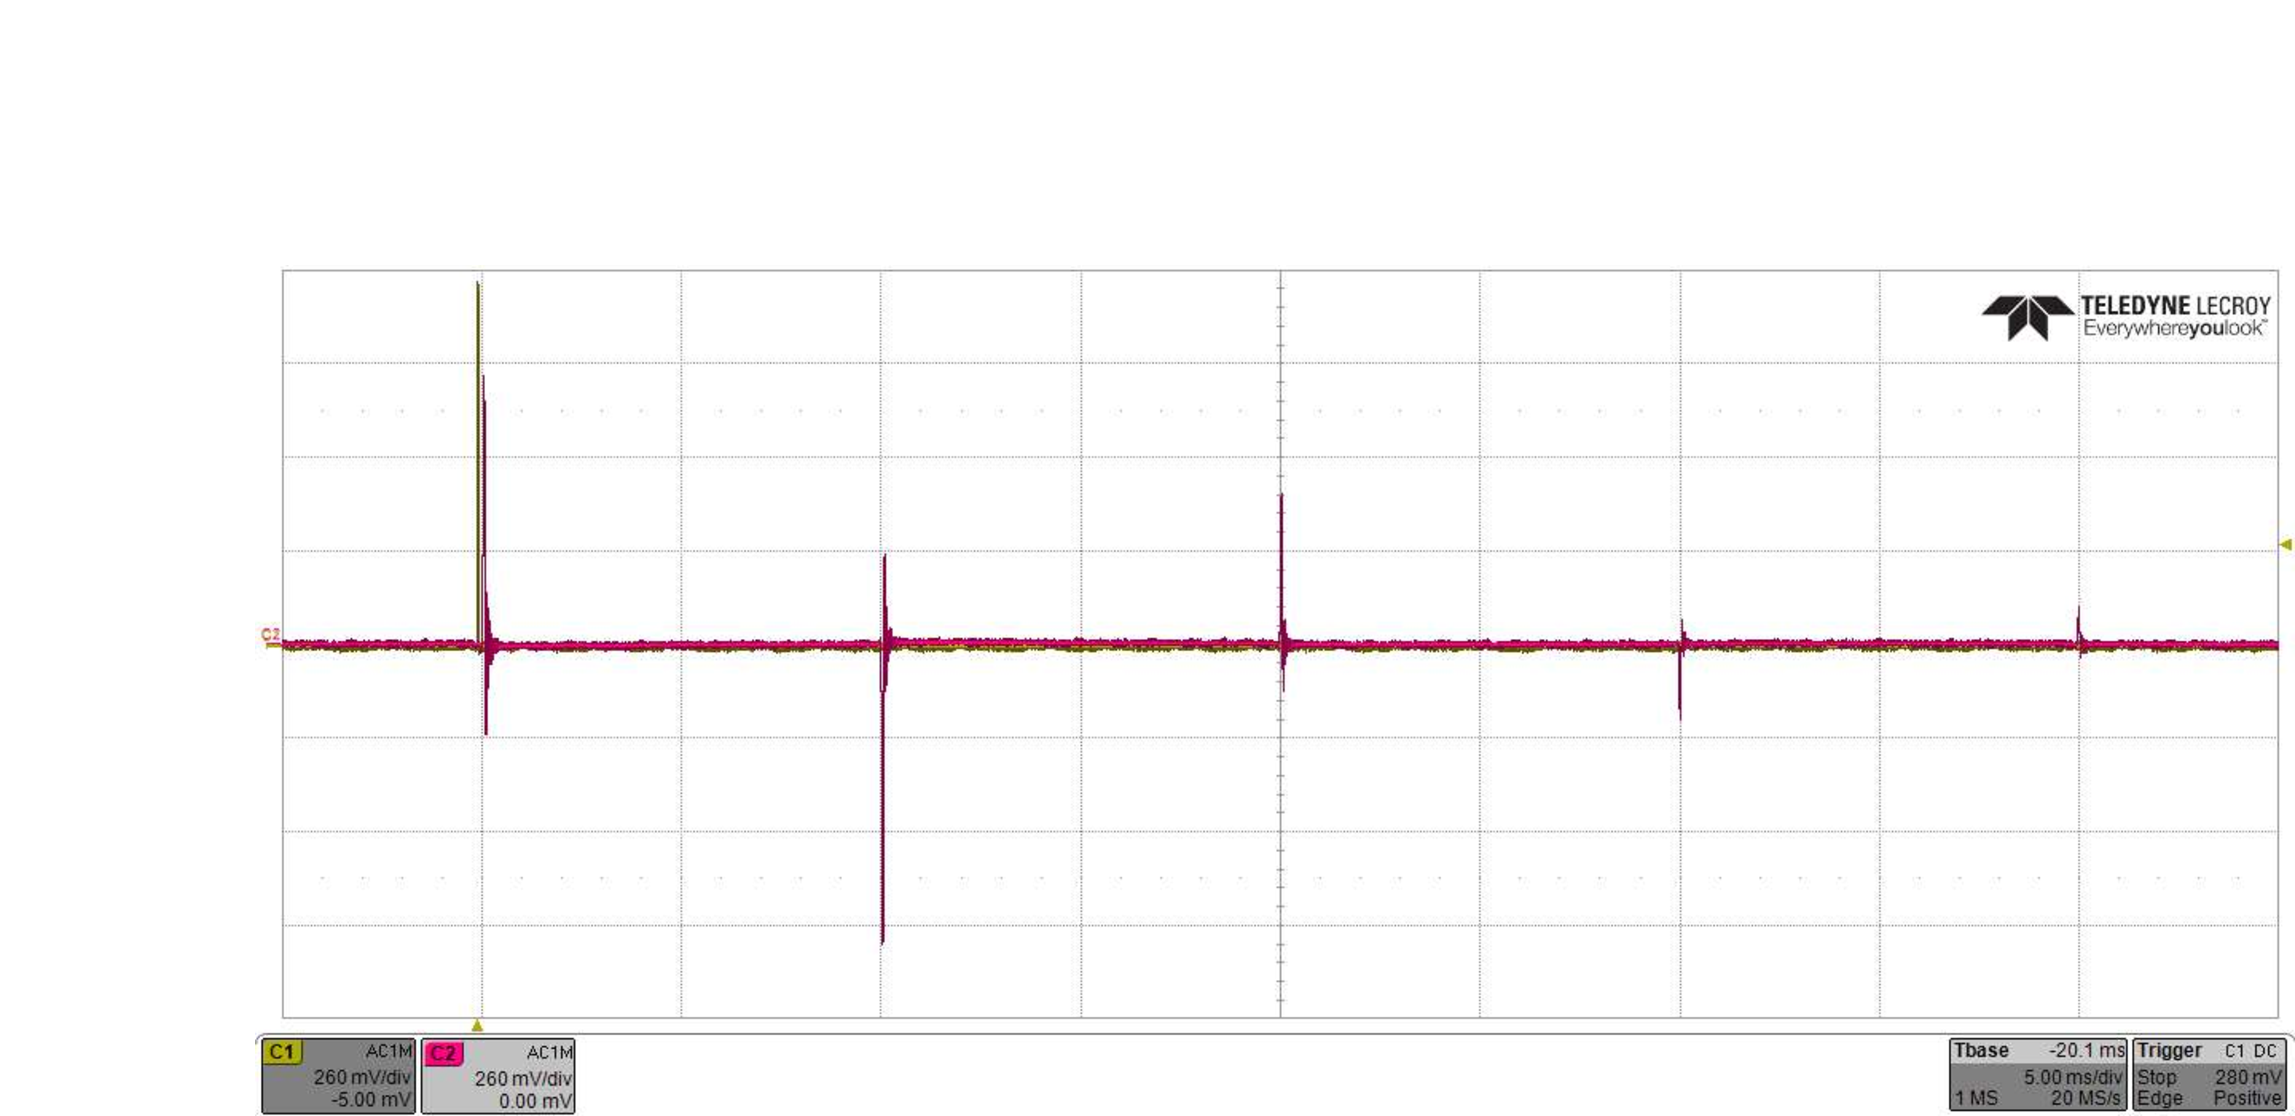
\includegraphics[width=0.9\textwidth, height=5cm]{billeder/reverb.png}
		\caption{Impulsrespons for reverbtesten.}
		\label{fig:imp_reverb}
	\end{minipage}\hfill
	\begin{minipage}{0.50\textwidth}
		\centering
		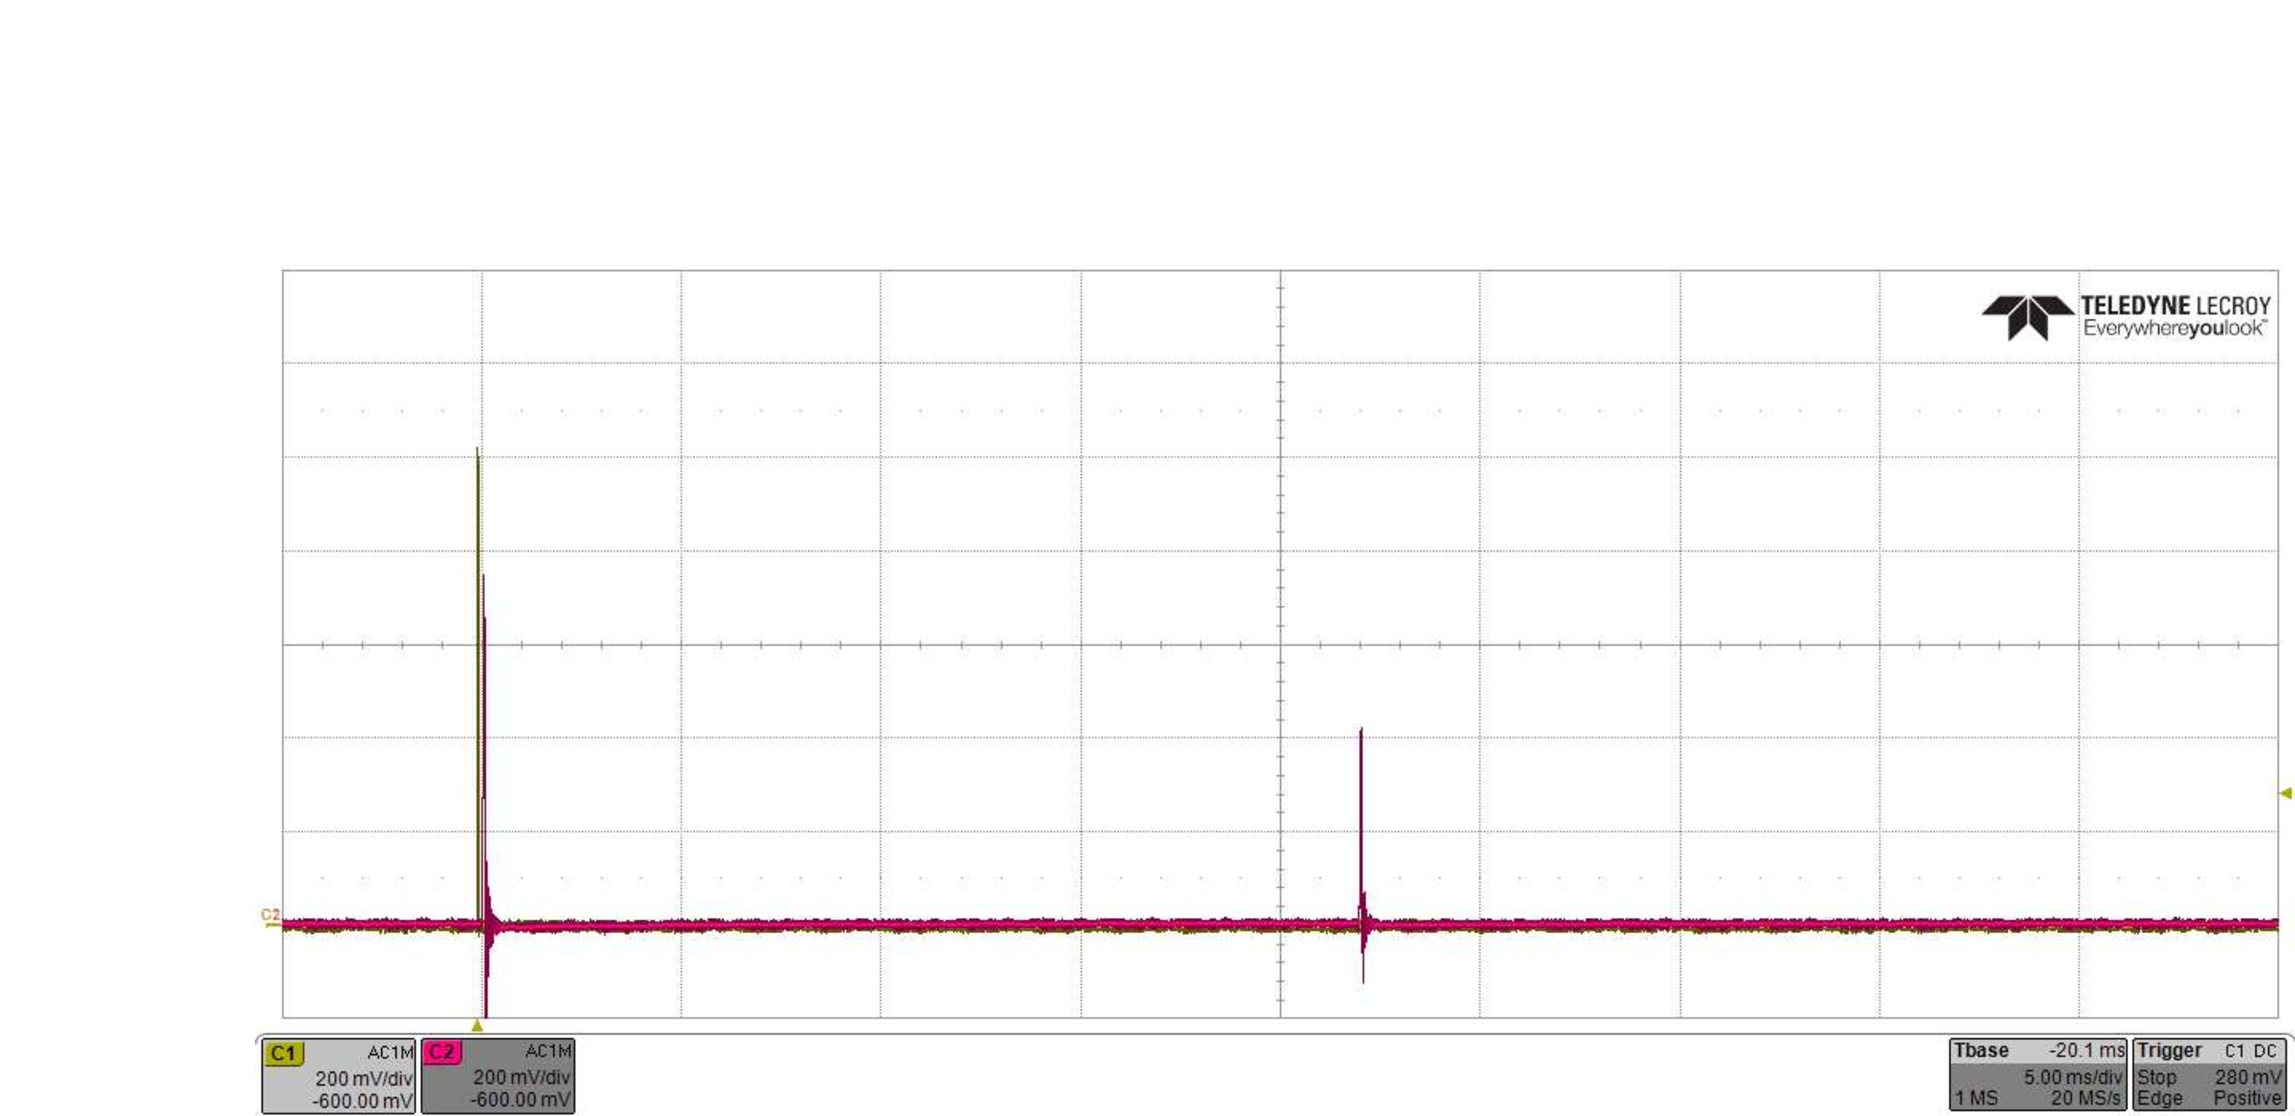
\includegraphics[width=0.9\textwidth, height=5 cm]{billeder/echo.png}
		\caption{Impulsrespons for echoeffekten.}
		\label{fig:imp_echo}
	\end{minipage}
\end{figure}
På figurene kan det aflæses at delay tiderne stemmer meget præcist overens med de fra programmets side forventede delay tider. På figuren for echo (\ref{fig:imp_echo}) ses også at gentagelsen af impulsen er faldet til ca $400\si{mV}$ hvor det oprindelige output er lige under $800\si{mV}$, hvilket stemmer nogenlunde overens med det forventede gain på $0.5$.\newline 
På reverb figuren (\ref{imp_reverb}) ses det at den første gentagelse af impulsen er af samme størrelse som det oprindelige output dette skyldes at feedforward har en gain på $0.5$ og feedback har samme gain så de udgør til sammen en fuld kopi af det oprindelige signal. 
Under normal brug vil disse gains være betydeligt lavere hvilket vil give et noget hurtigere aftagende respons men for at få et tydeligere test resultat blev disse ret høje gain værdier valgt.
%\husk{Sonny}{kan godt huske noget om at vi også testede på indgange til µControlleren, men var der ikke den samme støj på den almindelige indgang og vi ser den næsten heller ikke i matlab plottende}
%Støjen på indgangen skyldes de tre anti-aliasing filtre, som var forbundet via \husk{hvad kalder man de ting} hvilket giver en dårlig forbindelse.\newline
%
%\husk{Sonny}{Først målte tal så hvad de tilsvare præcis i "samples" og så kan der siges at det passer til det delay vi forventede}
%Her \ref{fig:impulsresponsreverb} ses impulsresponset af reverbeffekten.
%Som det fremgår af figuren bliver samplen gengivet med en dæmpning hver $2000$. sample.
%Gains samt delay var sat højt for at overdrive og tydeliggøre feedbacket.\newline
%Som det ses på figuren bliver impulsen feedbacket èn gang som svarende til et ekko efter $2000$ svarende til $45,35\si{mS}$.


\chapter{Ordliste} \label{bilag:ordliste}

\begin{table}[h!]
	\caption{Ordliste}
	\label{tab:ordliste}
	\begin{threeparttable}
		\begin{tabular}{l p{0.7\textwidth}}
			\toprule
			\textbf{Ord}      & \textbf{Beskrivelse}   \\ 
			\midrule
			AA			& Antialiasing.\\
			ADC			& Analog digital converter (Eng.)\\
			ANSI		& American National Standards Institute (Eng.)\\
			API			& Grænseflade på en computer der tillader én softwarekomponent at kommunikere med en anden\tnote{a}\\
%			CLI			& Commandline interface (Eng.)\\
			DAC			& Digital analog converter (Eng.)\\
%			Latency		& (Eng.) Tidsforsinkelsen imellem stimulans og respons.\\ 
			LCD			& Liquid crystal display (Eng.) \\
			MCU       	& Micro Controller Unit (Eng.). Microcontroller eller mikroprocessor. \\
%			Periferienhed & Selvkørende hardwaremodul i mikrocontrollerens arkitektur.\\
			Preemptive	& (Eng.) Afbrydelse af task fra fx. en scheduler.\\
			PWM			& Pulse Width Modulation (Eng.) \\
			SAR			& Successive Approximation Register (Eng.)\\
%			Shell		& Brugerinterface (CLI) til operativsystemets funktionalitet.\\
			SPI			& Serial Peripheral Interface (Eng.)  \\
			UART		& Universal asynchronous receiver and transmitter (Eng.)\\
			\bottomrule
		\end{tabular}
	
		\begin{tablenotes}
			\item[a] \textit{Den Danske Ordbog - \url{http://ordnet.dk/}}
		\end{tablenotes}
	\end{threeparttable}
\end{table}

%\input{section/symbol}
%\chapter{Pin mapping} \label{bilag:pinmap}
\begin{table}[h!]
	\centering
	\caption{Pin konfiguration af Tiva LaunchPad, EMP print og Projekt print}
	\label{tab:pin_mapping}
	\begin{threeparttable}
		\begin{tabular}{l l l l l l}
			\toprule
			\textbf{Tiva Pin\tnote{a}} 	& 
			\textbf{GPIO\tnote{b}}  	&
			\textbf{Tiva\tnote{c}} 		& 
			\textbf{EMP\tnote{d}}  		&
			\textbf{Projekt\tnote{e}} 	\\ 
			\midrule
			1.01 &      & 3V3  	& +3.3VDC		& 3V3		\\
			1.02 &  PB5 &      	& PB5			& (SPI2) FSS/$\overline{CS}$		\\
			1.03 &	PB0 &	   	& PB0			& Debug P0	\\
			1.04 &	PB1 &      	& PB1			& Debug	P1	\\
			1.05 &	PE4 &	   	& Audio Out     & Audio In Left	\\
			1.06 &	PE5 &	   	& Audio In		& Audio In Right \\
			1.07 &	PB4 &	   	& PB4			& (SPI2) CLK/SCK		\\
			1.08 &	PA5 &	   	& DIGI A		& 					\\
			1.09 &	PA6 &	   	& DIGI B    	& 								\\
			1.10 &	PA7 &	   	& DIGI P2		& 								\\
			\midrule
			2.01 &     	& GND  	& GND  			& GND 						\\
			2.02 & PB2 	&      	& T3CCP0 (PWM)	& 							\\
			2.03 & PE0 	&	  	& KEYB G 		&								\\
			2.04 & PF0 	& SW2	& 				&								\\
			2.05 &     	& RESET	& 				&								\\
			2.06 & PB7	&		& PB7			& (SPI2) TX/SDI					\\
			2.07 & PB6	&		& PB6			& (SPI2) RX (NA)				\\
			2.08 & PA4 	&      	& KEYB F 		&						\\
			2.09 & PA3 	&		& KEYB E    	& 						\\
			2.10 & PA2  &		& KEYB D		& 						\\
			\midrule
			3.01 &		& 5V0	& +5VDC			&	+5VDC							\\
			3.02 &		& GND	& GND			&	GND							\\
			3.03 & PD0	&(R10)	&				&								\\
			3.04 & PD1	&(R9)	&				&								\\
			3.05 & PD2	&		& LCD RS		& 				\\
			3.06 & PD3	&		& LCD E			& 						\\
			3.07 & PE1	&		& KEYB H		& 							\\
			3.08 & PE2	&		& KEYB J		&							\\
			3.09 & PE3	&		& KEYB K		&								\\
			3.10 & PF1	&LED (R)& LED R			&								\\
			\bottomrule
		\end{tabular}
	
		\begin{tablenotes}
			\item[] Forsættes på næste side...
		\end{tablenotes}
	\end{threeparttable}
\end{table}
\newpage
\begin{table}[ht]
	\centering
	\caption{Pin konfiguration af Tiva LaunchPad, EMP print og Projekt print}
	\begin{threeparttable}
		\begin{tabular}{l l l l l l}
			\toprule
			\textbf{Tiva Pin\tnote{a}} 	& 
			\textbf{GPIO\tnote{b}}  	&
			\textbf{Tiva\tnote{c}} 		& 
			\textbf{EMP\tnote{d}}  		&
			\textbf{Projekt\tnote{e}} 	\\ 
			\midrule
			4.01 & PF2	&LED (B)& LED Y			&								\\
			4.02 & PF3	&LED (G)& LED G			&								\\
			4.03 & PB3	&		& PB3			&	$\overline{LDAC}$							\\
			4.04 & PC4	&		& LCD D4		& 			\\
			4.05 & PC5	&		& LCD D5		& 				\\
			4.06 & PC6	&		& LCD D6		& 				\\
			4.07 & PC7	&		& LCD D7		& 				\\
			4.08 & PD6	&		& Status LED	& 		\\
			4.09 & PD7	&		& 				&								\\
			4.10 & PF4	& SW1	& 				&								\\
			\bottomrule
		\end{tabular}
		
		\begin{tablenotes}
			\item[x] Jumper på EMP printet skal sættes til. \textbf{J5 pin 1-2} og \textbf{J4} skal fjernes.
			\item[a,b] JP1-4 på Tiva LaunchPad \cite[Afsnit 2.1.5 s. 9]{spmu296}.
			\item[c] On-board funktion \cite[Afsnit 2.1.5 s. 9]{spmu296}.
			\item[d] EMP print funktionalitet er beskrevet i tilhørende diagram \cite{emp-diagram}.
			\item[e] Projekt , se bilag \ref{bilag:diagram}.
		\end{tablenotes}
	\end{threeparttable}
\end{table}
%\chapter{Stykliste} \label{bilag:styklister}
\begin{table}[h!]
\small
%\centering
\caption{Stykliste for diagrammet \ref{bilag:diagram}.}
\label{tab:styklister}
\begin{threeparttable}
\begin{tabular}{p{0.22\linewidth}p{0.1\linewidth}p{0.18\linewidth}p{0.05\linewidth}p{0.1\linewidth}p{0.1\linewidth}p{0.05\linewidth}}
%\begin{tabular}{ l l l l l l l }
\toprule
\multicolumn{1}{l}{\textbf{Komponent}}       &
\multicolumn{1}{l}{\textbf{Værdi}}       &
\multicolumn{1}{l}{\textbf{Type}}       &
\multicolumn{1}{l}{\textbf{Tol.}} &
\multicolumn{1}{l}{\textbf{Klasse}} &
\multicolumn{1}{l}{\textbf{Bemærkning}} &
\multicolumn{1}{l}{\textbf{Type / Lev.}}  \\ 
\hline
R1, R2, R4, R6, R7,& $\SI{47}{\kilo\ohm}$ & Keramisk SMD & $\pm 1\%$ & $\SI{0.25}{\watt}$ & 100ppm/\si{\celsius} & (c) \\
R9 &&&&&& \\
R3, R8 & $\SI{5}{\kilo\ohm}$ & Keramisk SMD	& $\pm 1\%$ & $\SI{0.25}{\watt}$ & 100ppm/\si{\celsius}  & (c) \\
R5, R10 & $\SI{100}{\kilo\ohm}$ & Potentiometer	& $\pm 1\%$ & $\SI{0.25}{\watt}$ & 100ppm/\si{\celsius}  & (c) \\
R11X*4, R12X*4, & $\SI{10}{\kilo\ohm}$ & Keramisk SMD	& $\pm 1\%$ & $\SI{0.25}{\watt}$ & 100ppm/\si{\celsius}  & (c) \\
R21X*4, R22X*4, &&&&&& \\
R31X*4, R32X*4 &&&&&& \\
\midrule
C1, C2, C4, C5 & $\SI{490}{\nano\farad}$ & Keramisk SMD & $\pm 5\%$ & 100 \si{\volt} &  & (c)\\
C3, C6, C15X*4, & $\SI{0,1}{\micro\farad}$ & Keramisk SMD & $\pm 5\%$ & 100 \si{\volt} &  & (c)\\
C25X*4, C35X*4 &&&&&&\\
C7, C8 & $\SI{1}{\micro\farad}$ & Keramisk SMD & $\pm 5\%$ & 100 \si{\volt} &  & (c)\\
C2U1 & $\SI{10}{\micro\farad}$ & Keramisk SMD & $\pm 5\%$ & 100 \si{\volt} &  & (c)\\
C2U2 & $\SI{100}{\nano\farad}$ & Keramisk SMD & $\pm 5\%$ & 100 \si{\volt} &  & (c)\\
C11X*4, C33X*4 & $\SI{220}{\pico\farad}$ & Keramisk SMD & $\pm 5\%$ & 100 \si{\volt} &  & (c)\\
C12X*4, C37X & $\SI{100}{\pico\farad}$ & Keramisk SMD & $\pm 5\%$ & 100 \si{\volt} &  & (c)\\
C13X*4 & $\SI{470}{\nano\farad}$ & Keramisk SMD & $\pm 5\%$ & 100 \si{\volt} &  & (c)\\
C14X*4, C17X*4, & $\SI{2,2}{\nano\farad}$ & Keramisk SMD & $\pm 5\%$ & 100 \si{\volt} &  & (c)\\
C18X*4, C22X*4 &&&&&& \\
C16X*4, C28X*4 & $\SI{470}{\pico\farad}$ & Keramisk SMD & $\pm 5\%$ & 100 \si{\volt} &  & (c)\\
C21X*4, C23X*4, & $\SI{47}{\nano\farad}$ & Keramisk SMD & $\pm 5\%$ & 100 \si{\volt} &  & (c)\\
C32X*4 &&&&&& \\
C24X*4, C34X*4, & $\SI{1}{\nano\farad}$ & Keramisk SMD & $\pm 5\%$ & 100 \si{\volt} &  & (c)\\
C36X*4 &&&&&&\\
C26X*4, C27X*4, & $\SI{15}{\pico\farad}$ & Keramisk SMD & $\pm 5\%$ & 100 \si{\volt} &  & (c)\\
C38X*4, C39X*4 &&&&&&\\
C29X*4 & $\SI{4,7}{\nano\farad}$ & Keramisk SMD & $\pm 5\%$ & 100 \si{\volt} &  & (c)\\
C31X*4 & $\SI{10}{\nano\farad}$ & Keramisk SMD & $\pm 5\%$ & 100 \si{\volt} &  & (c)\\
\midrule
IC5*4, IC6*4, IC7*4, IC11, IC12 & AD8031 & OP Amp &  &  &  & (a) \\
U1 & MCP4922-E/P & DAC &  &  &  & (d) \\
SV1, SV2 & TM4C123GH6PM & &  &  &  & (b) \\
X\textunderscore IN & KLBR4 & & & & Surface mount & (e) \\
X\textunderscore OUT & KLBR4 & & & & Surface mount & (e) \\
\hline
\bottomrule
\end{tabular}
\begin{tablenotes}
%\textbf{Typ/Lev.}
\item[a] (), (Analog Devices)
\item[b] (), (Texas Instruments, http://www.ti.com/lit/ds/symlink/tm4c123gh6pm.pdf)
\item[c] (), (Phillips)
\item[d] (), (Microchip)
\item[e] (), (Lumberg)
\item[u] Ukendt
\end{tablenotes}
\end{threeparttable}
\end{table} 

%\input{section/tidsplan}
%\input{section/diagrammer}
%\chapter{Diagram} \label{bilag:diagram} % Denne side skal ikke bruges, den skal blot fjernes og erstattes med digrammet


\end{document}
